%%%%%%%%%%%%%%%%%%%%%%%%%%%%%%%%%%%%%%%%%
% University Assignment Title Page 
% LaTeX Template
% Version 1.0 (27/12/12)
%
% This template has been downloaded from:
% http://www.LaTeXTemplates.com
%
% Original author:
% WikiBooks (http://en.wikibooks.org/wiki/LaTeX/Title_Creation)
%
% License:
% CC BY-NC-SA 3.0 (http://creativecommons.org/licenses/by-nc-sa/3.0/)
% 
% Instructions for using this template:
% This title page is capable of being compiled as is. This is not useful for 
% including it in another document. To do this, you have two options: 
%
% 1) Copy/paste everything between \begin{document} and \end{document} 
% starting at \begin{titlepage} and paste this into another LaTeX file where you 
% want your title page.
% OR
% 2) Remove everything outside the \begin{titlepage} and \end{titlepage} and 
% move this file to the same directory as the LaTeX file you wish to add it to. 
% Then add \input{./title_page_1.tex} to your LaTeX file where you want your
% title page.
%
%%%%%%%%%%%%%%%%%%%%%%%%%%%%%%%%%%%%%%%%%
%\title{OpenNAS tutorial}
%----------------------------------------------------------------------------------------
%	PACKAGES AND OTHER DOCUMENT CONFIGURATIONS
%----------------------------------------------------------------------------------------

\documentclass[12pt]{article}
\usepackage[english]{babel}
\usepackage[utf8x]{inputenc}
\usepackage{amsmath}
\usepackage{graphicx}
\usepackage[colorinlistoftodos]{todonotes}
\usepackage{hyperref}
\usepackage{xcolor}
\usepackage{subcaption}
\usepackage{float}

\begin{document}

\begin{titlepage}

\newcommand{\HRule}{\rule{\linewidth}{0.5mm}} % Defines a new command for the horizontal lines, change thickness here

\center % Center everything on the page
 
%----------------------------------------------------------------------------------------
%	HEADING SECTIONS
%----------------------------------------------------------------------------------------

\textsc{\LARGE University of Sevilla}\\[1.5cm] % Name of your university/college
\textsc{\Large Architecture and Technology of Computers Dept.}\\[0.5cm] % Major heading such as course name
\textsc{\large Robotics and Technology of Computers Lab.}\\[0.5cm] % Minor heading such as course title

%----------------------------------------------------------------------------------------
%	TITLE SECTION
%----------------------------------------------------------------------------------------

\HRule \\[0.4cm]
{ \huge \bfseries OpenNAS for dummies}\\[0.4cm] % Title of your document
\HRule \\[1.5cm]
 
%----------------------------------------------------------------------------------------
%	AUTHOR SECTION
%----------------------------------------------------------------------------------------

\begin{minipage}{0.4\textwidth}

\begin{flushleft} \large
\emph{Authors:}\\
Daniel \textsc{Gutierrez} \\ % Your name
Juan Pedro \textsc{Dominguez} \\
Angel \textsc{Jimenez} \\
Alejandro \textsc{Linares}
\end{flushleft}
\end{minipage}
~
%\begin{minipage}{0.4\textwidth}
%\begin{flushright} \large
%emph{Supervisor:} \\
%Angel \textsc{Jimenez} \\ % Supervisor's Name
%Alejandro \textsc{Linares}
%\end{flushright}
%\end{minipage}\\[2cm]

% If you don't want a supervisor, uncomment the two lines below and remove the section above
%\Large \emph{Authors:}\\
%Daniel \textsc{Gutierrez}\\[3cm] % Your name

%----------------------------------------------------------------------------------------
%	DATE SECTION
%----------------------------------------------------------------------------------------
\vfill % Fill the rest of the page with whitespace
{\large \today}\\[2cm] % Date, change the \today to a set date if you want to be precise

%----------------------------------------------------------------------------------------
%	LOGO SECTION
%----------------------------------------------------------------------------------------
\begin{center}

\includegraphics[width=0.8\textwidth]{logo.png}\\[1cm] % Include a department/university logo - this will require the graphicx package
\end{center}


 
%----------------------------------------------------------------------------------------

\vfill % Fill the rest of the page with whitespace

\end{titlepage}


\begin{abstract}
OpenNAS is a software tool to customize, create, and generate a Neuromorphic Auditory Sensor (NAS) model ready to be loaded within the FPGA-based AER-Node board. It is the result of many research years in the field of neuromorphic engineering, in which our research group has enough experience. As its name indicates, this spike-based auditory sensor tries to mimic the human ear and the way in which it works. OpenNAS can be divided in three main blocks: the input, where the sound is obtained, digitized and converted into spikes; the spike-based audio processing step, where the input spikes are decomposed into frequency channels, and, finally, the output stage, where the output interface through which the spikes are going to be sent is selected. Since there is not a standard "cochlea configuration", OpenNAS tool offers the possibility to set a large set of parameters with the aim of providing the best approach for the required spike-based audio applications.
\end{abstract}

\section{Introduction}
\label{sec:Introduction}
%----------------------------------------------------------------------------------------
%	NAS original paper
%----------------------------------------------------------------------------------------
\textit{``This paper presents a new architecture, design flow and FPGA implementation analysis of a neuromorphic binaural auditory sensor, designed completely in the spike-domain. Unlike digital cochleae that decompose audio signals using classical Digital Signal Processing (DSP) techniques, the model presented in this paper processes information directly encoded as spikes using Pulse Frequency Modulation (PFM) and provides a set of frequency-decomposed audio information using an Address-Event Representation (AER) interface. In this case, a systematic approach to design led to a generic process for building, tuning and implementing audio frequency decomposers with different features, facilitating synthesis with custom features. This allows researchers to implement their own parameterized neuromorphic auditory systems in a low cost FPGA in order to study the audio processing and learning activity that takes place in the brain. In this paper we present a 64 channel binaural neuromorphic auditory system implemented in a Virtex-5 FPGA using a commercial development board. The system was excited with a diverse set of audio signals in order to analyze its response and characterize its features. The neuromorphic auditory system response times and frequencies are reported. The experimental results of the proposed system implementation with 64 channels stereo are: frequency range between 9.6Hz to 14.6KHz (adjustable), maximum output event rate of 2.19Mevents/sec, power consumption of 29.7mW, slices requirements of 11,141 and system clock frequency of 27MHz."} 

%----------------------------------------------------------------------------------------
%	Spike-based Signal Processing blocks experience
%----------------------------------------------------------------------------------------

This paragraph belongs to the NAS \cite{jimenez2017binaural} original paper (its abstract). At the beginning, the idea was to design, develop and test spike-base processing blocks, which we called building blocks, to offer the community a way to develop more complex spike-based systems. We succeed in the development of spike-based motor controllers and spike-based filters.

Spike-based motor control blocks implement complex operations. However, in the spike domain, those operations are easier to solve than using the classical methods. One example of this simplification could be... Basic operations, like additions and subtractions were also implemented in the spike-domain. More information about how those operations work can be found in \cite{jimenez2010building}.
%\todo{Under development}

%----------------------------------------------------------------------------------------
%	NAS motivation
%----------------------------------------------------------------------------------------

One of the most important spike-based block designed in this work was the band-pass filter, because it allowed to implement a filter bank, and then, to decompose a input signal into different frequency bands. It made it possible to work on our own Neuromorphic Auditory Sensor. The inspiration was taken from important authors as Lyon \cite{lyon1988analog}, among others, who developed bio-inspired analog cochlea model.

\begin{figure}[H]
  \centering
  \begin{minipage}[b]{0.8\textwidth}
    \centering
    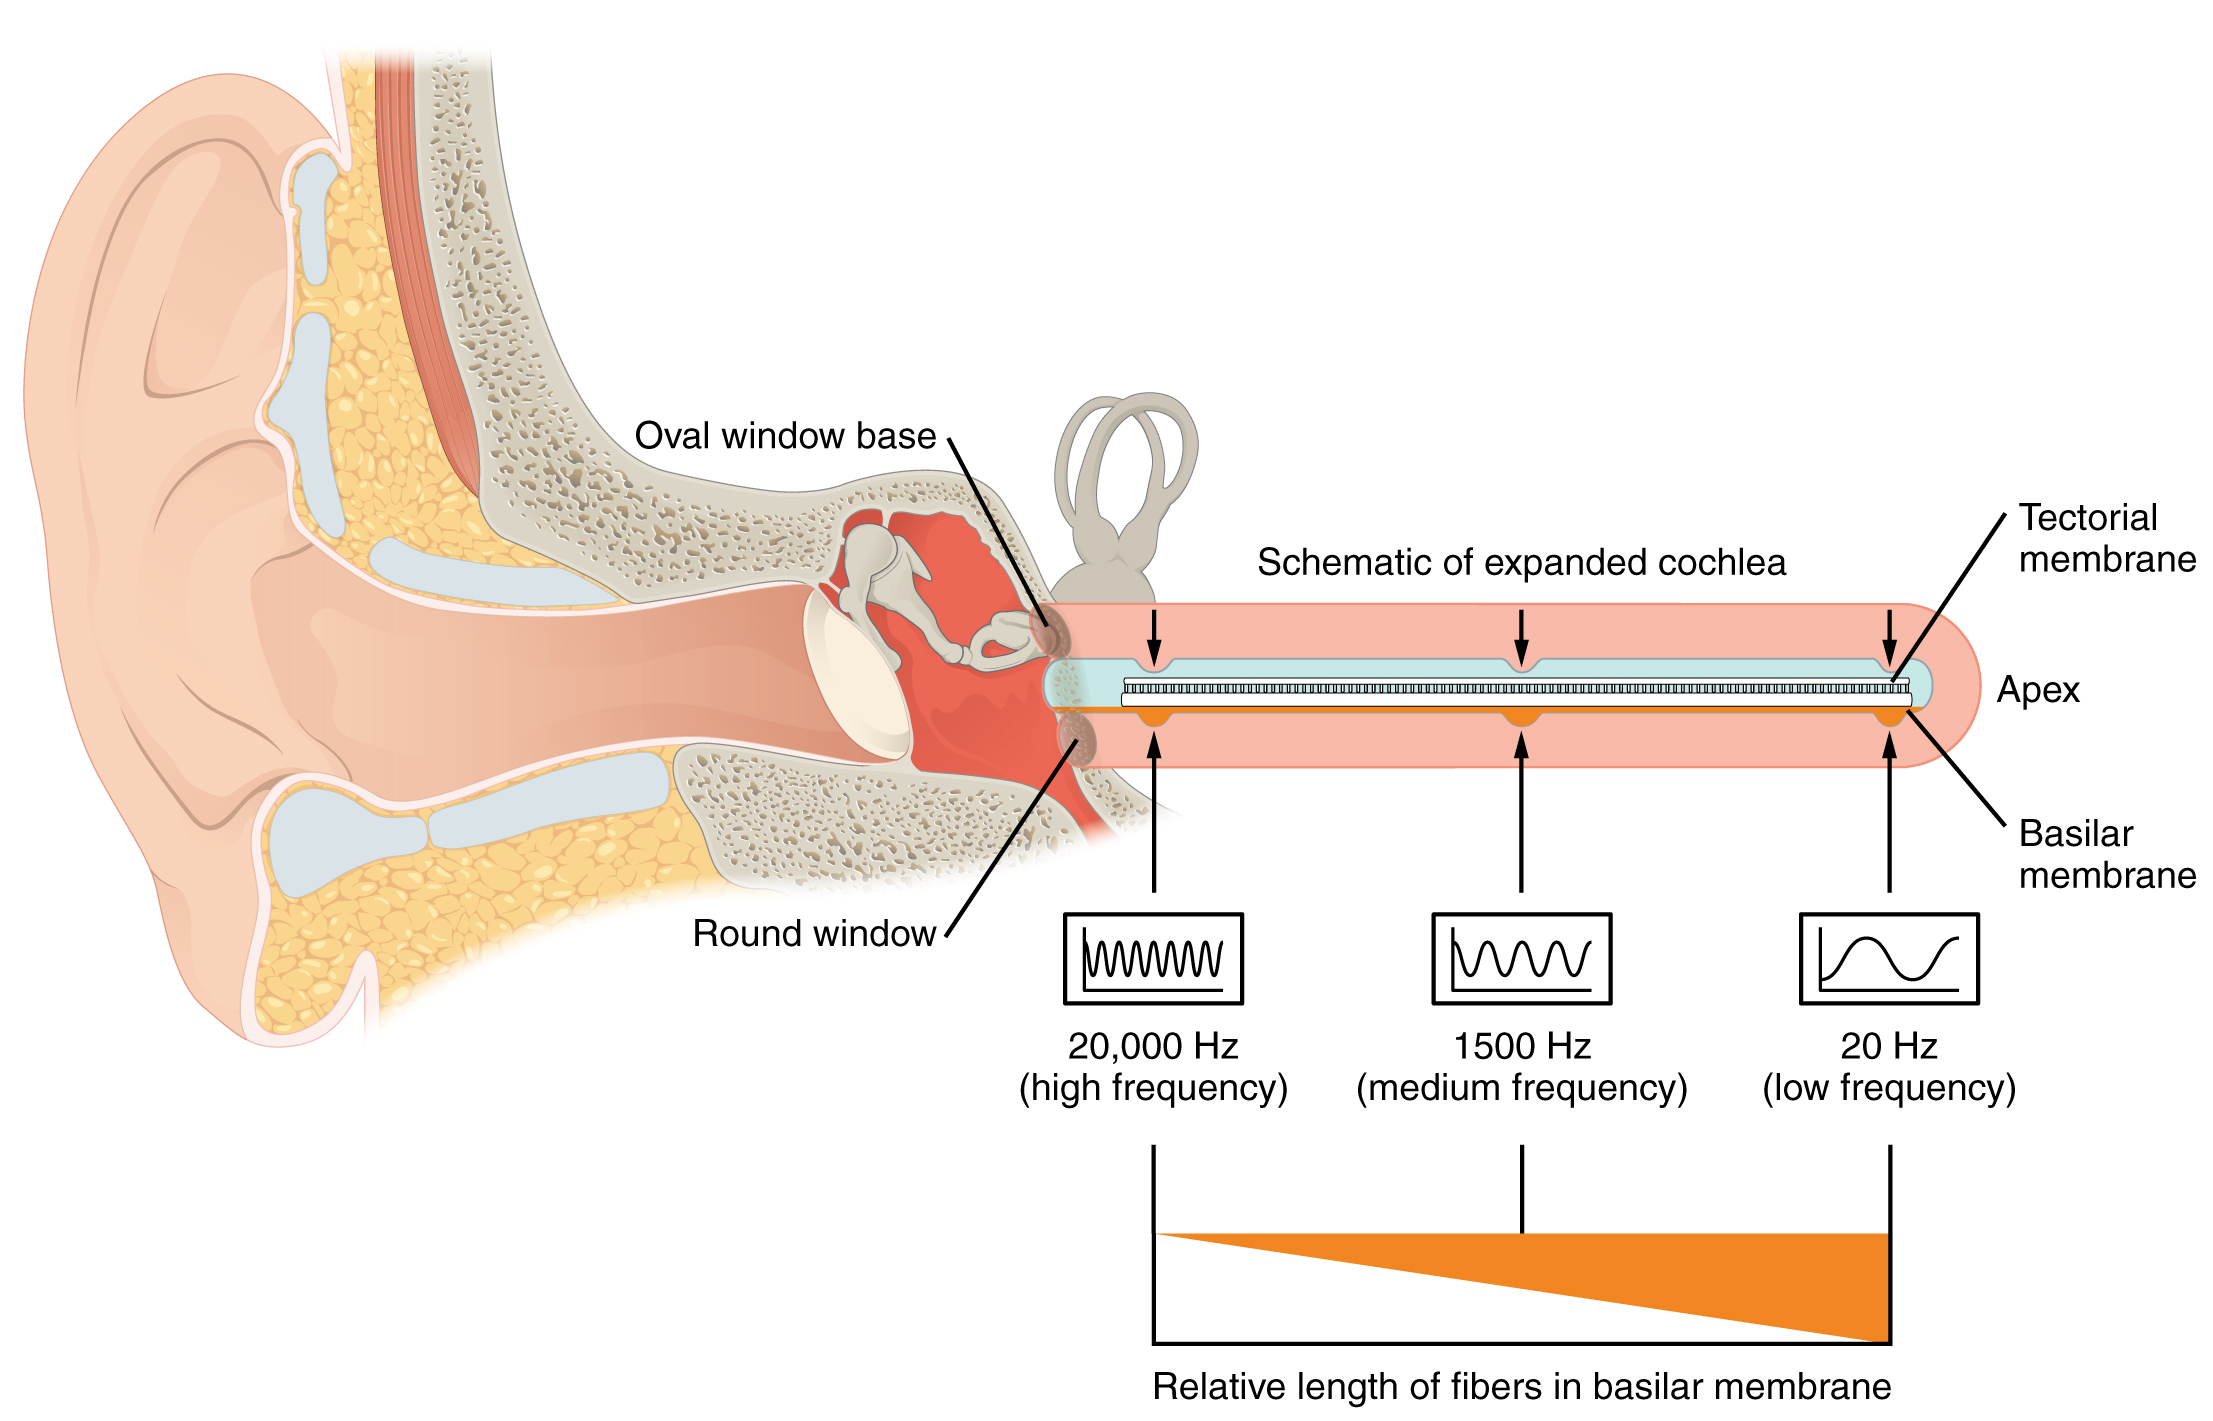
\includegraphics[width=1\textwidth]{biological_ear_model.jpg}
    %\caption{Picture 1}
    \label{fig:biological_model}
  \end{minipage}
  \\%
  \begin{minipage}[b]{1\textwidth}
    \centering
    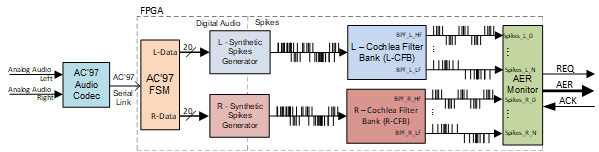
\includegraphics[width=1\textwidth]{NAS_Block_Diagram.png}
    \caption{Top: biological model of human ear. Bottom: NAS architecture block diagram.}
    \label{fig:nas_block_diagram}
  \end{minipage}
\end{figure}


%----------------------------------------------------------------------------------------
%	What did we develop?
%----------------------------------------------------------------------------------------

As a complex system, and based on the state of the art, the NAS is composed by several spike-based processing blocks, and it could be separated into three well differentiated and independent parts:
\begin{itemize}
\item Audio Input,
\item Processing stage,
\item Output interface.
\end{itemize}

%Decir que se ha hecho el nas para ahorrar tiempo debido a que es para fpga y \todo[inline, color=green!40]{tienes que instanciar todos los bloauqes a mano.}

And don't be afraid if the NAS doesn't work as you hope. You will have infinite tries to get the perfect one! :)

%----------------------------------------------------------------------------------------
%	Now, we are able to...
%----------------------------------------------------------------------------------------

By using OpenNAS software, the user will be able to configure each of those three parts separately. The tool has been developed to easily configure and generate........ 

%----------------------------------------------------------------------------------------
%	Future works
%----------------------------------------------------------------------------------------

\section{OpenNAS overview}
\label{sec:Overview}

\subsection{Requirements}

\begin{itemize}
    \item \textbf{SOFTWARE}: First of all, we need to check some software requirements to be sure that OpenNAS tool is going to work properly. All the software packages belong to Microsoft .NET Framework. Therefore, we will need a \textbf{Microsoft Windows OS} version running in the computer (Windows7 or Windows10). If you are not a Windows user (probably because you prefer a Linux distribution), you will need a Virtual Machine (VM) and a Windows installation. Furthermore, you should download the needed software. As IDE, \textbf{Visual Studio} was used since it provides an easy way to design Graphical User Interfaces (GUI) for Microsoft Windows OS. We will also need an specific framework, which includes features used in our software tool. More specific, we need to download and install both \textbf{.NET Framework 4.0} and \textbf{.NET Framework 4.5}.One of the best advantages that OpenNAS provides is the capacity of automatically generating the FPGA programming file (.bit extension) without either configure or create any project. This option is useful for people who are not familiarized with VHDL design. But, independently of what you need, you have to install \textbf{Xilinx ISE or Vivado} (depending of the board that you use). For the AER-Node board (device by default), you will need ISE. For the rest, Vivado for Xilinx FPGA chips (supported by OpenNAS); or Intel Quartus Prime Design Software for Altera FPGA chips (not supported yet).Finally, since we are going to use a specific manufacturer, you will also need a proprietary software to download the programming file into the FPGA board. \textbf{iMPACT} allows you either programming the FPGA using the RAM memory (volatile option) or the FLASH memory (non-volatile option). It is usually installed at the same time that ISE is being installed. But if not, you can go to the Xilinx Download Center website and download the software.
    
    \item \textbf{HARDWARE}: About the hardware requirements, you can use your own boards, but we can not offer any guaranties about the system operation. If you are interested on to use our neuromorphic hardware, please visit the \textcolor{blue}{\href{https://www.t-cober.es}{COBER}} web site and check the neuromorphic hardware catalog.
    
\end{itemize}




\textbf{IMPORTANT NOTES:}
\begin{enumerate}
\item Versions are important: you must be sure that your installed software versions can support the OpenNAS project. Here there is a list which indicates the needed versions to run OpenNAS:
    \begin{itemize}
        \item Microsoft Windows OS: Windows7, Windows8 or Windows10.
        \item Visual Studio: Visual Studio 2015 or latest.
        \item .NET Framework: you will need two: .NET Framework 4.0 and .NET Framework 4.5
        \item Xilinx ISE Design Suite: ISE 14.7 \textbf{(It needs to support Spartan6 family chip)}
        \item Xilinx Vivado: any version of Vivado.
        \item Xilinx iMPACT: along with the ISE installation file.
    \end{itemize}
\item More important things coming soon...
\end{enumerate}

%\subsection{Software architecture}


\subsection{Design flow}

%Use the table and tabular commands for basic tables --- see Table~\ref{tab:widgets}, for example. You can upload a figure (JPEG, PNG or PDF) using the files menu. To include it in your document, use the includegraphics command as in the code for Figure~\ref{fig:frog} below.

%\begin{table}
%\centering
%\begin{tabular}{l|r}
%Item & Quantity \\\hline
%Widgets & 42 \\
%Gadgets & 13
%\end{tabular}
%\caption{\label{tab:widgets}An example table.}
%\end{table}

\begin{figure}[H]
\centering
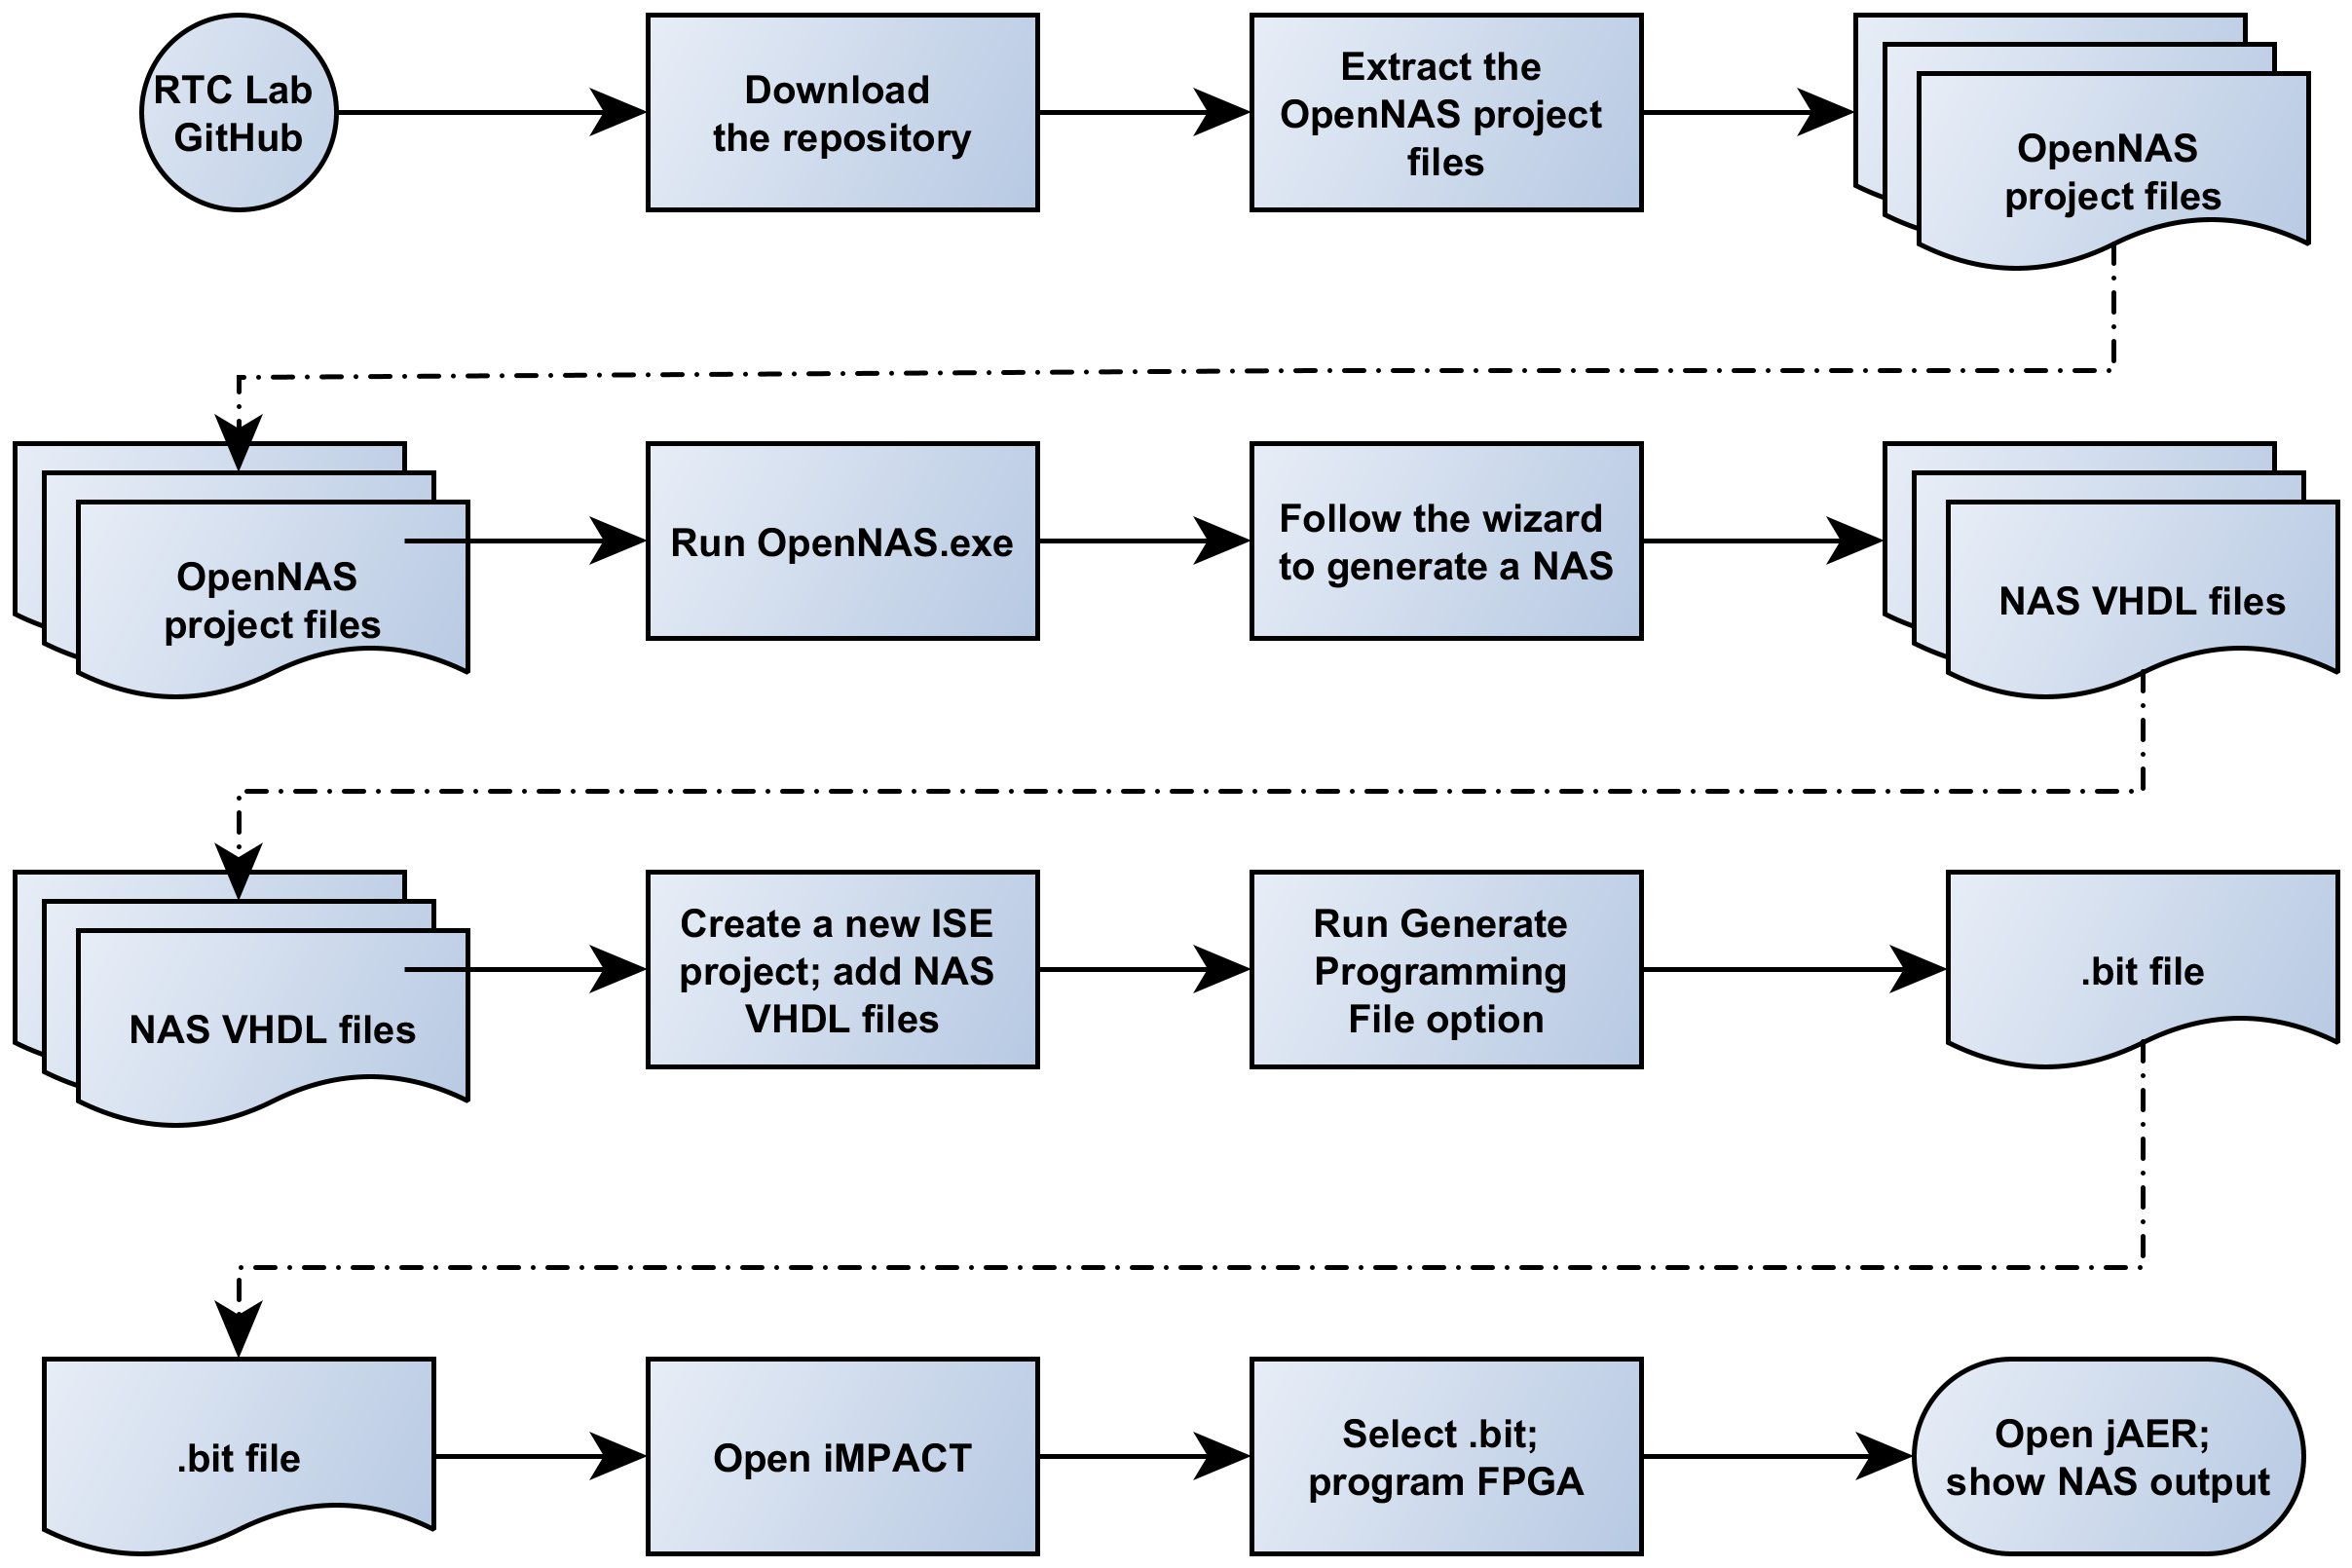
\includegraphics[width=0.8\textwidth]{NAS_design_flow.jpg}
\caption{\label{fig:nas_designflow}Complete design flow to work with NAS, starting from the GitHub repository to showing the NAS output by jAER.}
\end{figure}

\subsection{OpenNAS configuration options}

%You can make lists with automatic numbering \dots
%\begin{enumerate}
%\item Like this,
%\item and like this.
%\end{enumerate}
%\dots or bullet points \dots
%\begin{itemize}
%\item Like this,
%\item and like this.
%\end{itemize}

%\subsection{SSP blocks features}

%\LaTeX{} is great at typesetting mathematics. Let $X_1, X_2, \ldots, X_n$ be a sequence of independent and identically distributed random variables with $\text{E}[X_i] = \mu$ and $\text{Var}[X_i] = \sigma^2 < \infty$, and let
%$$S_n = \frac{X_1 + X_2 + \cdots + X_n}{n}
      %= \frac{1}{n}\sum_{i}^{n} X_i$$
%denote their mean. Then as $n$ approaches infinity, the random variables $\sqrt{n}(S_n - \mu)$ converge in distribution to a normal $\mathcal{N}(0, \sigma^2)$.

\subsubsection{Commons}

\begin{itemize}
    \item NAS Chip
        \begin{enumerate}
            \item AERNODE
            \item ZTEX
            \item SOCDOCK
            \item OTHER
        \end{enumerate}
    \item NAS Type 
        \begin{enumerate}
            \item MONO
            \item STEREO
        \end{enumerate}
    \item Number of Ch.
        \begin{itemize}
            \item Minimun: 2; Maximun: infinite; Recommendable: values that are 2-pow, as 8, 16, 32, 64, 128 or 256.
        \end{itemize}
    \item Clock Freq. (MHz)
        \begin{itemize}
            \item Depend of your target board.
        \end{itemize}
\end{itemize}

\subsubsection{Input}

\begin{itemize}
    \item Select Audio Input:
        \begin{enumerate}
            %----------------------
            % AC'97 Codec
            %----------------------
            \item AC'97 Codec
                \begin{itemize}
                    \item Audio Input
                        \begin{itemize}
                            \item LINE\_IN
                            \item MIC\_IN
                        \end{itemize}
                    \item Select Spikes Generator Settings
                        \begin{itemize}
                            \item Spikes Gen bits
                            \item Spikes Gen Clock Div
                            \item KspikesGen (GSpk./s)
                            \item Max Spike Rate: (KSpk./s)
                        \end{itemize}
                \end{itemize}
            %----------------------
            % I2S Audio ADC
            %----------------------
            \item I2S Audio ADC
                \begin{itemize}
                    \item Select Spikes Generator Settings
                        \begin{itemize}
                            \item Spikes Gen bits
                            \item Spikes Gen Clock Div
                            \item KspikesGen (KSpk./s)
                            \item Max Spike Rate: (KSpk./s)
                        \end{itemize}
                \end{itemize}
            %----------------------
            % PDM Mic
            %----------------------
            \item PDM Mic
                \begin{itemize}
                    \item PDM Settings
                        \begin{itemize}
                            \item System Clock (MHz)
                            \item PDM Clock Div
                            \item PDM Clock (MHz)
                        \end{itemize}
                    \item Anti-Offset SHPF Settings
                        \begin{itemize}
                            \item Cutt-off Freq. (Hz)
                        \end{itemize}
                    \item Anti-Aliasing SLPF Settings
                        \begin{itemize}
                            \item Cut-off Freq. (Hz)
                            \item Gain (dB)
                        \end{itemize}
                \end{itemize}
            %----------------------
            % I2S + PDM
            %----------------------
            \item I2S + PDM Mic
                \begin{itemize}
                    \item This option contains all the parameters listed before.
                \end{itemize}
        \end{enumerate}
\end{itemize}


\subsubsection{Processing}

\begin{itemize}
    \item Select NAS Architecture
        \begin{enumerate}
            \item Cascade SLPF Architecture
            
            \item Parallel SLPF Architecture
            
            \item Parallel SBPF Architecture
            
        \end{enumerate}
    
    \item SLPF Filter: only when either Cascade SLPF Architecture or Parallel SLPF Architecture is selected.
        \begin{enumerate}
            \item Order 2
        \end{enumerate}
    
    \item Number of Channels
    
    \item Start Freq. (Hz): according to the human ear, should be 20 Hz.
    
    \item Stop Freq. (Hz): according to the human ear, should be 22 KHz.
    
    \item SBPF Q Factor: only when Parallel SBPF Architecture is selected.
    
    \item SBPF Output Att. (dB)
    
    \item Target Mid Frequencies (Hz)
    
    \item SLPF Cut-off Frequencies (Hz)
    
    \item SBPF Q Factor: only when Parallel SBPF Architecture is selected.
    
    \item SBPF Attenuation (dB)
    
\end{itemize}

\subsubsection{Output}

\begin{itemize}
    \item Select Spikes Output
        \begin{enumerate}
            \item Spikes Distributed Monitor
                \begin{itemize}
                    \item Spikes Distributed Monitor
                        \begin{itemize}
                            \item Spikes to monitor
                            \item Spikes FIFO Bits
                            \item AER FIFO Bits
                            \item Total Bits
                        \end{itemize}
                \end{itemize}
            \item SpiNNaker-AER Interface v1
            
            \item SpiNNaker-AER Interface v2
            
            \item SpiNNaker-AER Interface v1 + Spikes Distributed Monitor
            
            \item USB Interface
            
        \end{enumerate}
\end{itemize}

\section{OpenNAS wizard: how to use step by step}
\label{sec:Steps}

At this point, we are ready to start using the OpenNAS software tool. Maybe, you now can think "Did I not ready before to read about spike-based signal processing?" Well, for getting started you do not need to be a professional on that topic, but if your target is to implement complex systems, it would be good to know how the NAS works.

We will split the tutorial to use OpenNAS in three parts: first we need to download the project from the NAS GitHub web page. After that, we have to either run the OpenNAS .exe file or open the OpenNAS VisualStudio project, in order to follow the OpenNAS wizard. And finally, to create an ISE project to generate the programming file needed to be loaded into the FPGA. 

Let's do it!

\subsection{OpenNAS GitHub repository}

%----------------------------------------------------------------------------------------
%	GitHub website
%----------------------------------------------------------------------------------------

First, click on the \textcolor{blue}{ \href{https://github.com/RTC-research-group/OpenNAS}{OpenNAS GitHub}} website. If the link does not work, you can also open a web browser, and then copy there the OpenNAS GitHub website link: https://github.com/RTC-research-group/OpenNAS.

\begin{figure}[H]
\centering
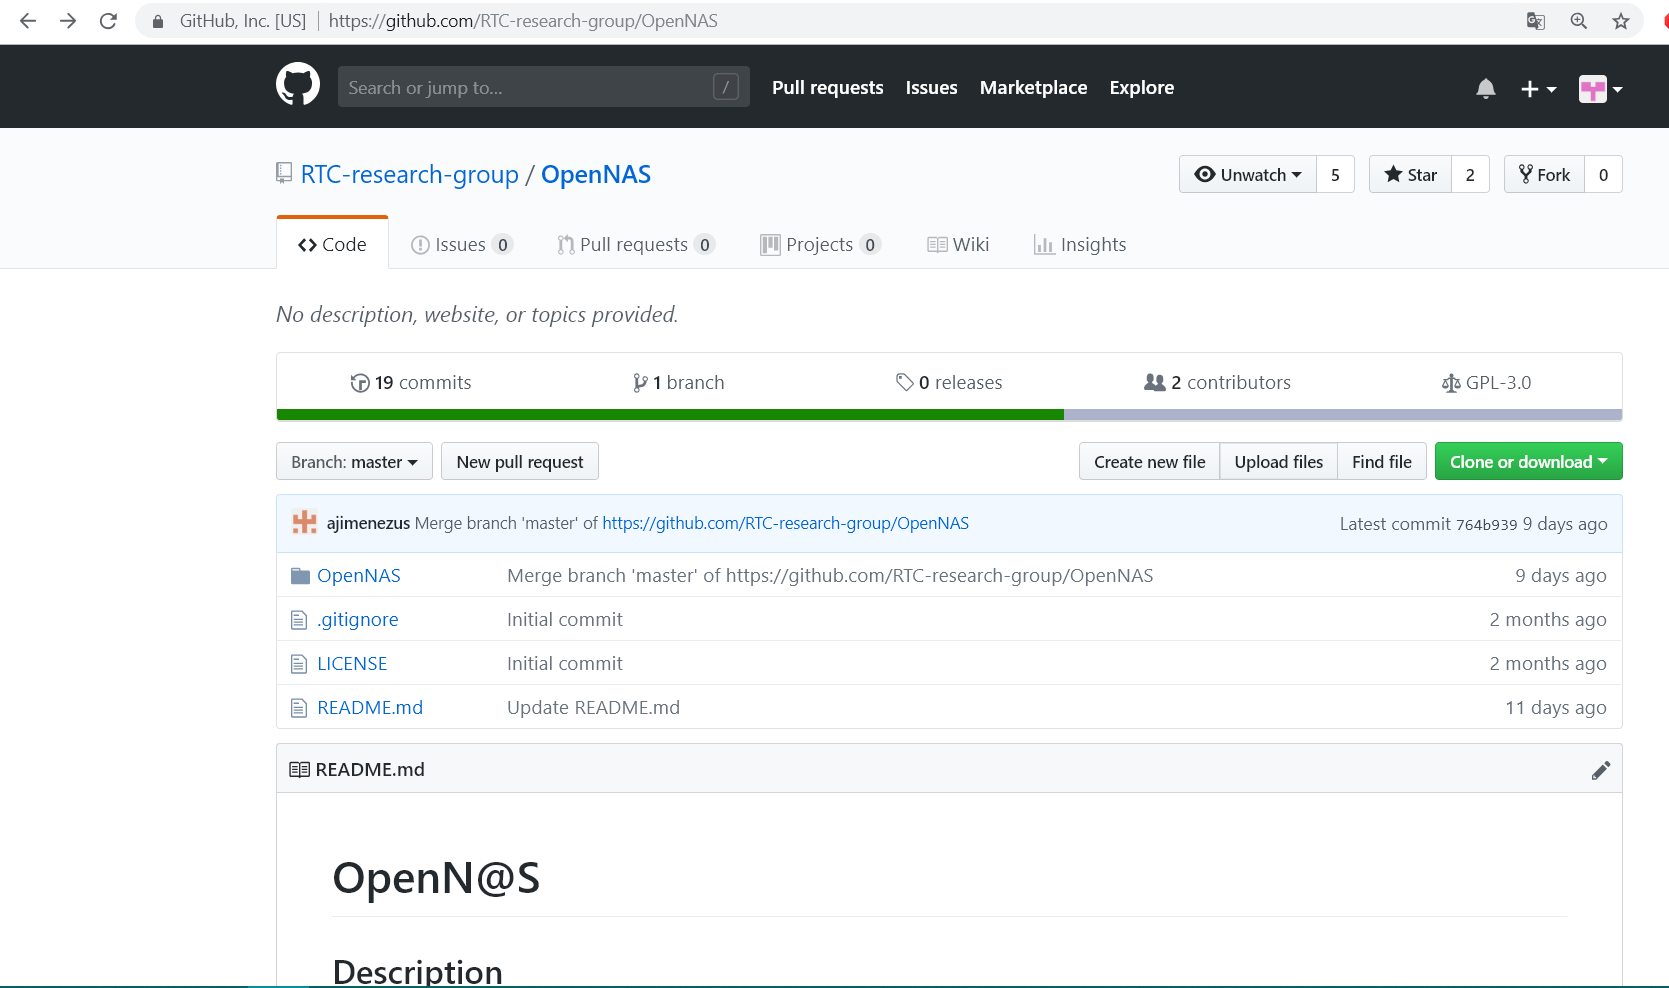
\includegraphics[width=1\textwidth]{images/Img01_OpenNAS_GitHub.PNG}
\caption{\label{fig:OpenNAS_repo}OpenNAS GitHub repository.}
\end{figure}

If that link does not work either, try to navigate to the RTC research group and look for the OpenNAS repository (https://github.com/RTC-research-group). There you can find a useful tool set to work with AER-based devices.

\begin{figure}[H]
\centering
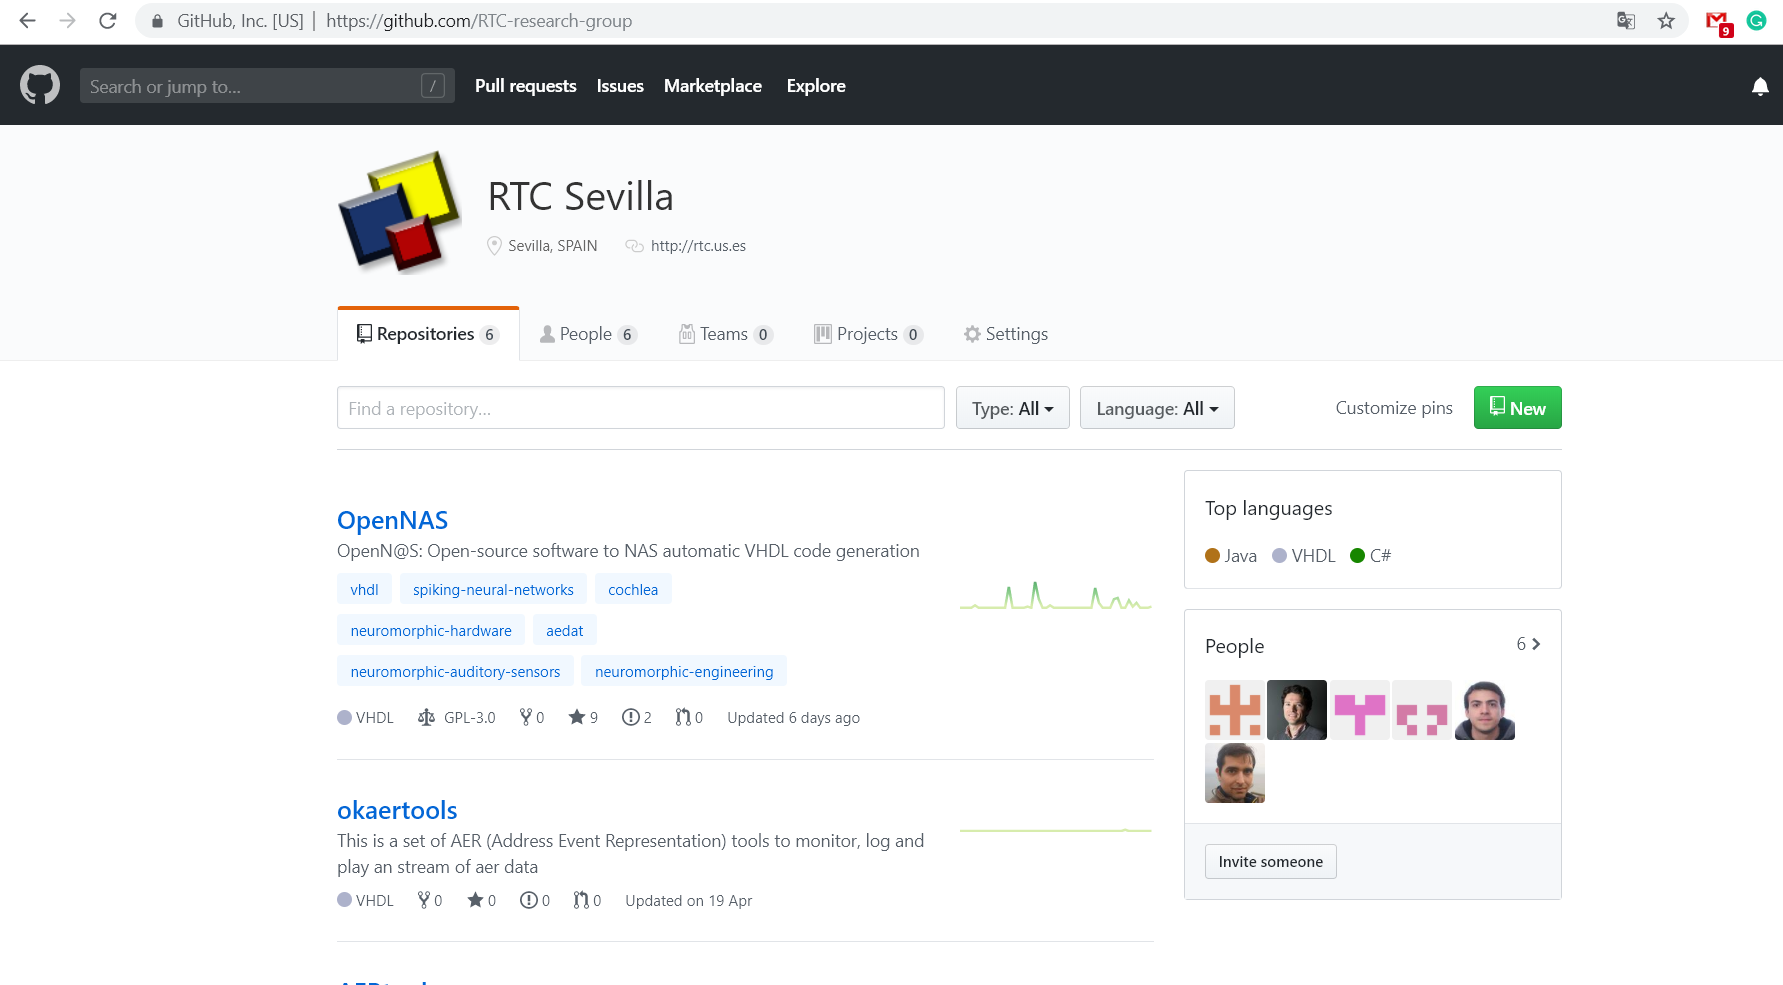
\includegraphics[width=1\textwidth]{images/Img00_RTC_GitHub.PNG}
\caption{\label{fig:RTC_GitHub_page}Robotics and Technology of Computers Lab. (RTC) GitHub page.}
\end{figure}

Once you are in the OpenNAS repository, there you can find a short wiki/tutorial about what is OpenNAS, how to getting started, how to use, how to contribute and, of course, how to cite our work. For us is very important the citations, so don't be shy. That wiki will be useful, but you can find more detailed information in this user manual.

\begin{figure}[H]
\centering
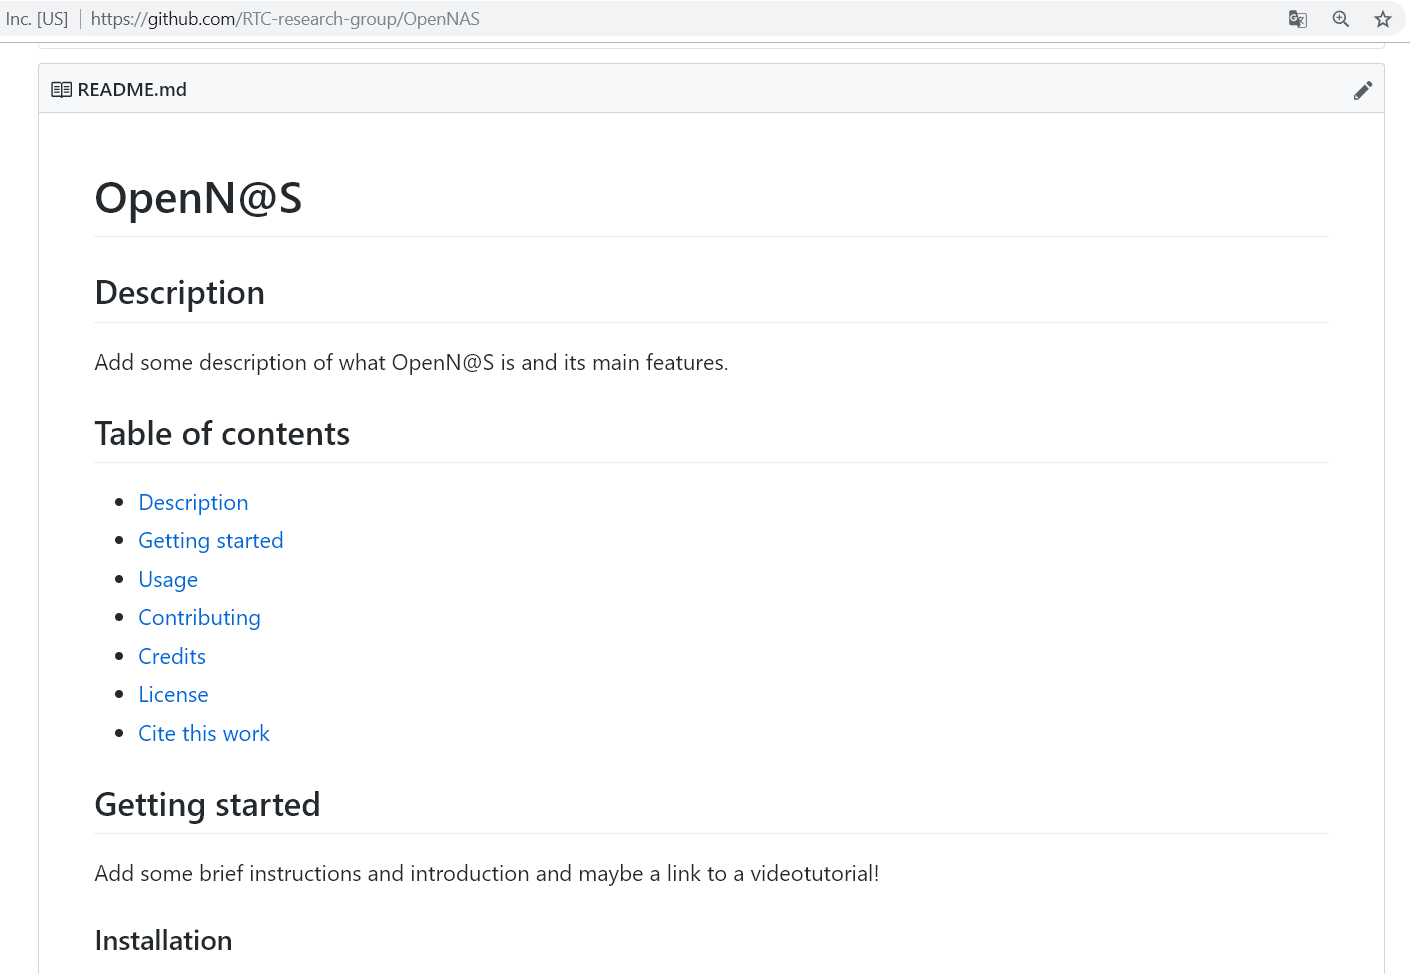
\includegraphics[width=1\textwidth]{images/Img02_OpenNASWiki_GitHub.PNG}
\caption{\label{fig:OpenNAS_wiki}OpenNAS wiki overview.}
\end{figure}

The next step is either to download the project in your computer or to clone it. It depends on what do you prefer. And feel free if you want to contribute. You will be welcome!

\begin{figure}[H]
\centering
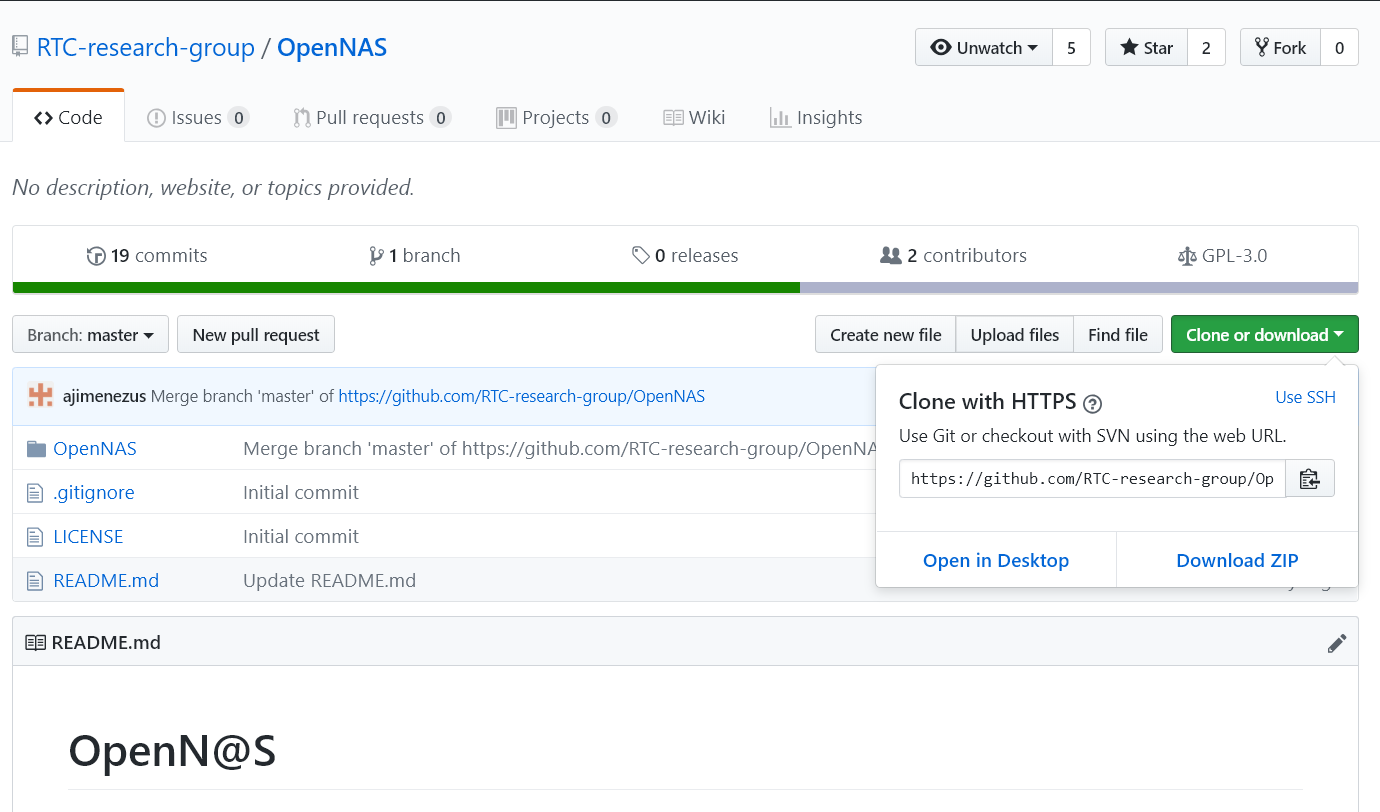
\includegraphics[width=1\textwidth]{images/Img03_Clone_DownloadOpenNAS.PNG}
\caption{\label{fig:Download_clone_OpenNAS_repo}How to either clone or download the OpenNAS GitHub repository.}
\end{figure}

If you take a look within OpenNAS main folder, there are several sub-folders which contain .VHD files (for FPGA) and .cs files (for C\# application). The software hierarchy has been explained more detailed in section "Software architecture".

\begin{figure}[H]
\centering
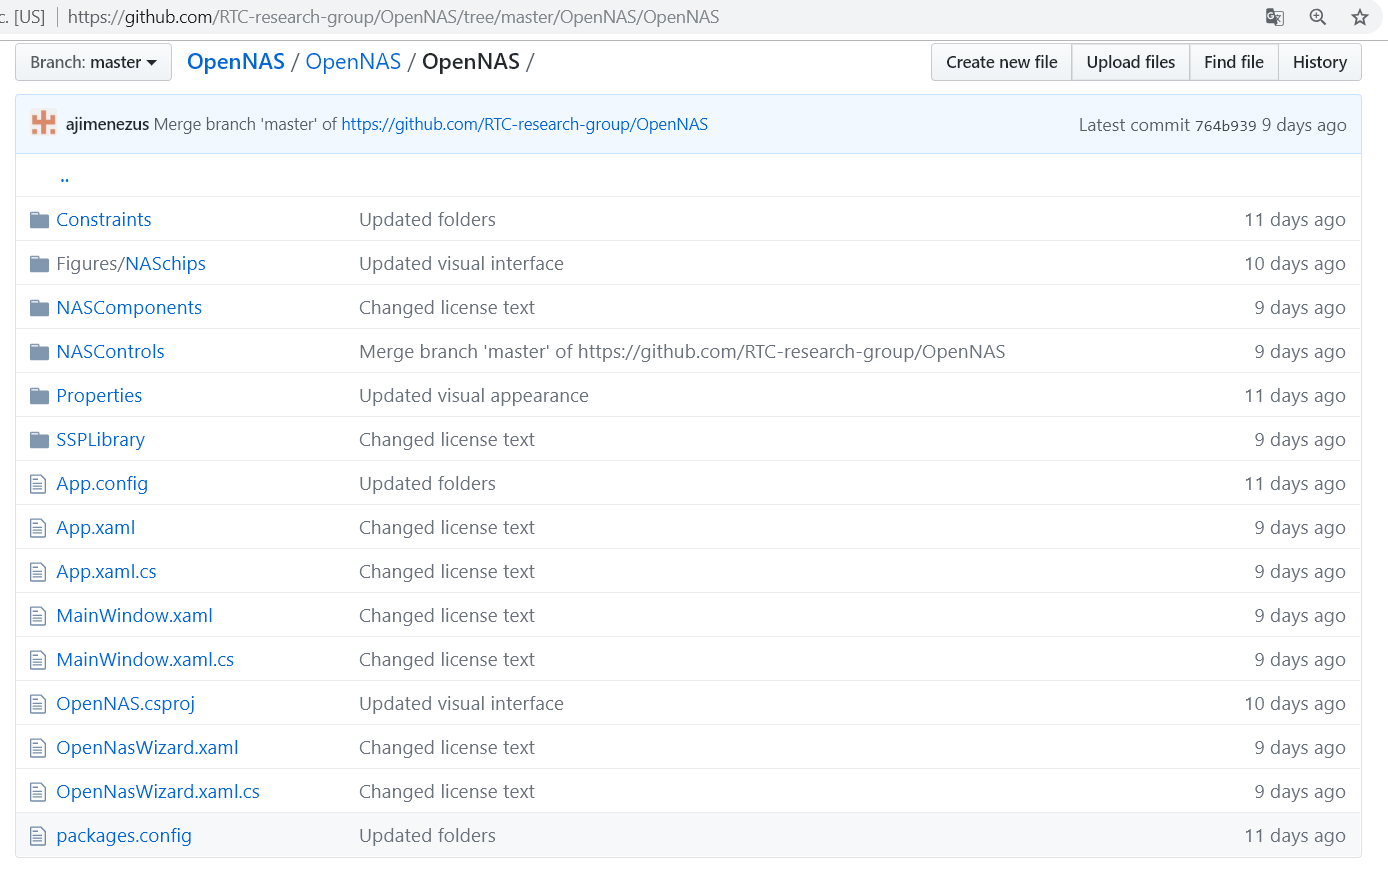
\includegraphics[width=1\textwidth]{images/Img04_OpenNAS_Project_Folders.PNG}
\caption{\label{fig:OpenNAS_folders}OpenNAS main folders.}
\end{figure}

Constraints folder is an important folder. It contains the files that you need to have well configured to use the NAS in your FPGA-based board. By default, OpenNAS includes three specific constraint files for three different boards: AER-Node board, SOC DOCK board, and ZTEX 2.13 board. If another board will be used, you must have to set your own constraint file. 

\begin{figure}[H]
\centering
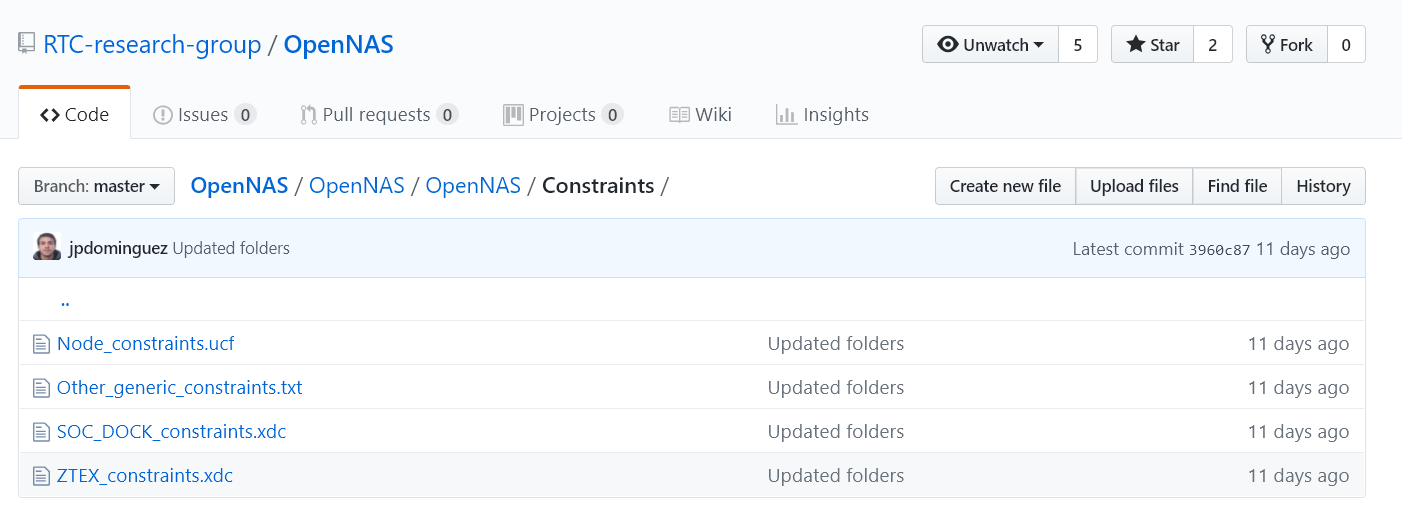
\includegraphics[width=1\textwidth]{images/Img05_Constraints.PNG}
\caption{\label{fig:OpenNAS_Constraints}Constraints files available from OpenNAS.}
\end{figure}

\textbf{Take care with that! This file is the main errors source.}

Related with the VHDL files, the SSP (Spike-based Signal Processing) folder contains all of the source code of the NAS. You should not modify those files, otherwise NAS could not work properly. But you can check how the NAS has been implemented using HDL code. 

\begin{figure}[H]
\centering
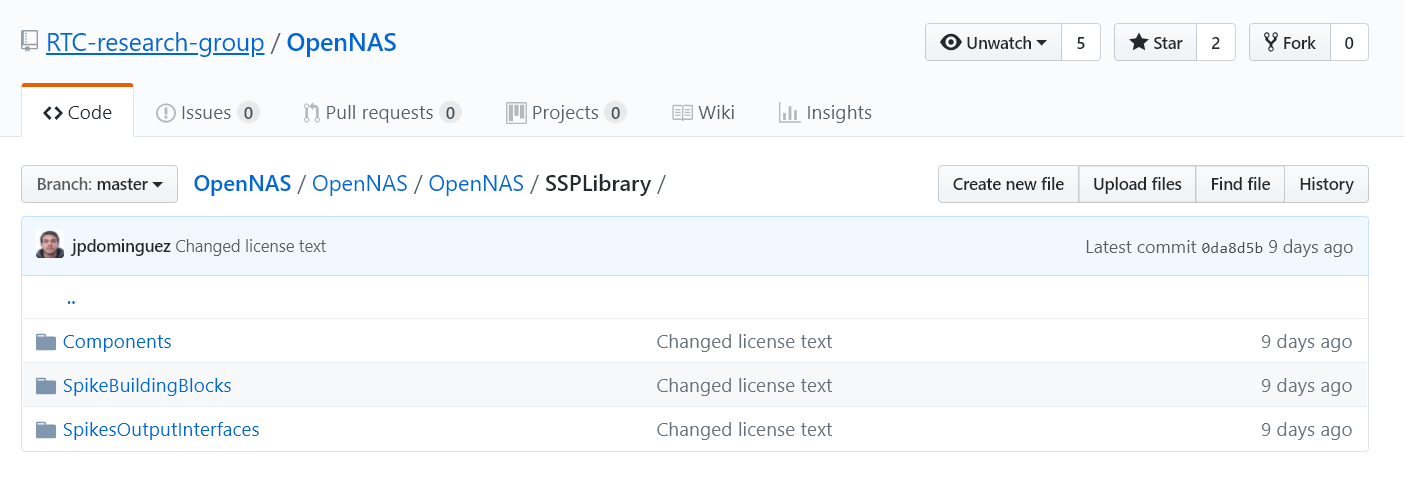
\includegraphics[width=1\textwidth]{images/Img06_SSP.PNG}
\caption{\label{fig:OpenNAS_SSPFolder}SSP folder contains all the NAS VHDL files.}
\end{figure}

Now, just a quick view of how those files look in the GitHub repository. This was showed clearly in the Software Architecture section.

\begin{figure}[H]
\centering
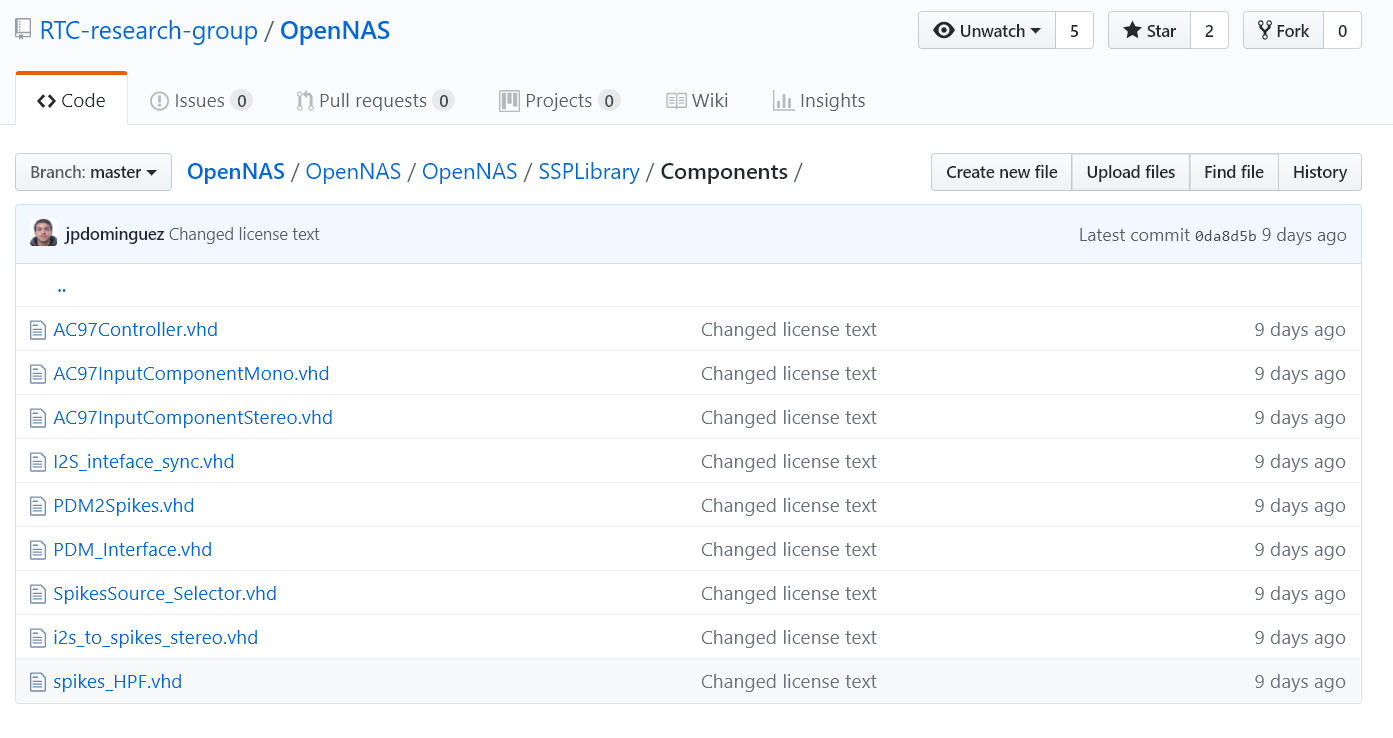
\includegraphics[width=1\textwidth]{images/Img07_Components.PNG}
\caption{\label{fig:OpenNAS_SSP_Components}NAS input VHDL modules.}
\end{figure}

\begin{figure}[H]
\centering
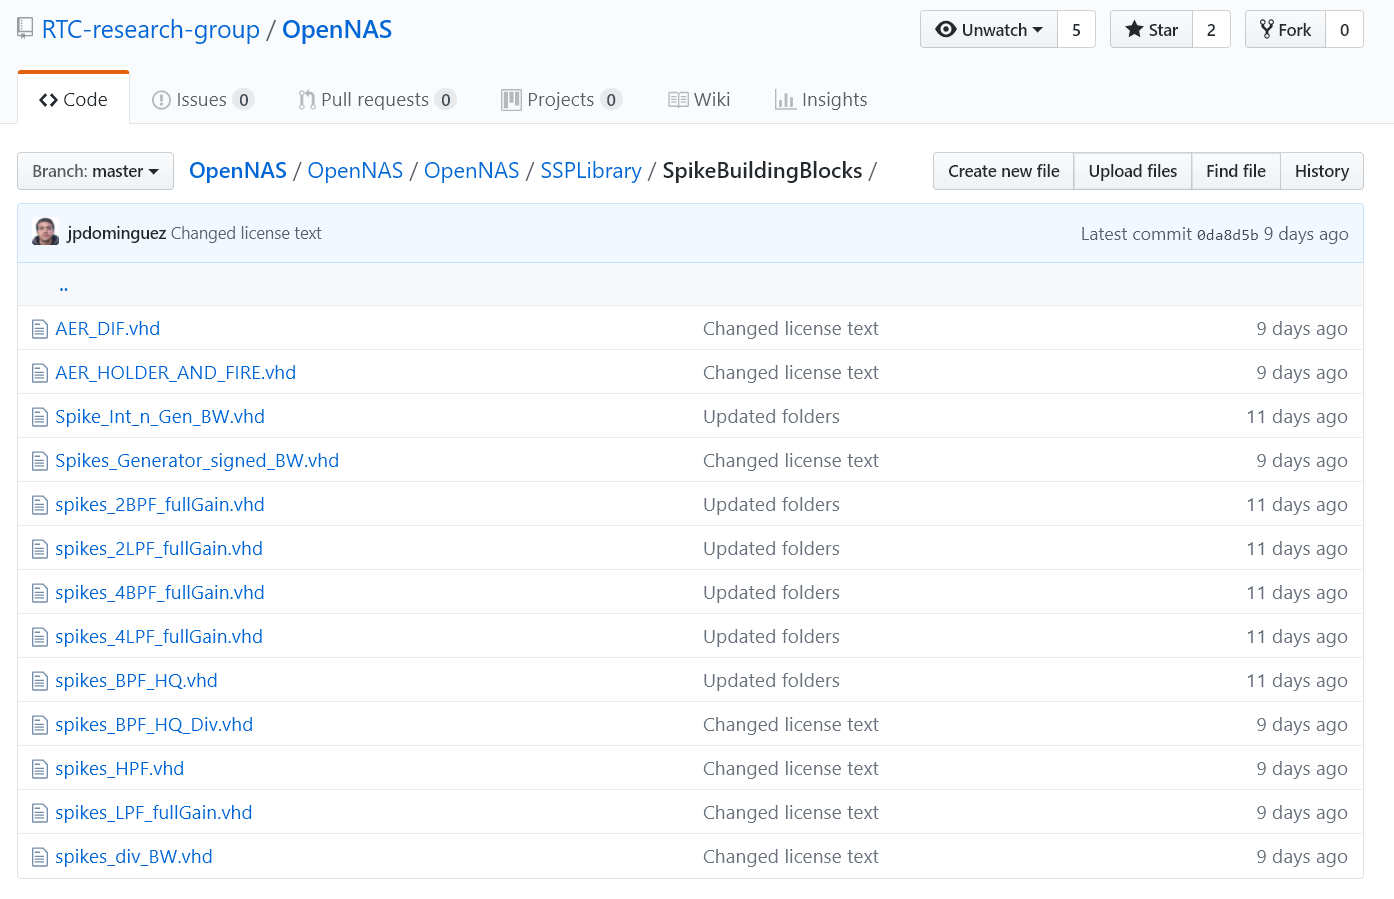
\includegraphics[width=1\textwidth]{images/Img08_SpikeBuildingBlocks.PNG}
\caption{\label{fig:OpenNAS_SSP_SpikesBuildingBlock}NAS spike-based signal processing VHDL modules.}
\end{figure}

\begin{figure}[H]
\centering
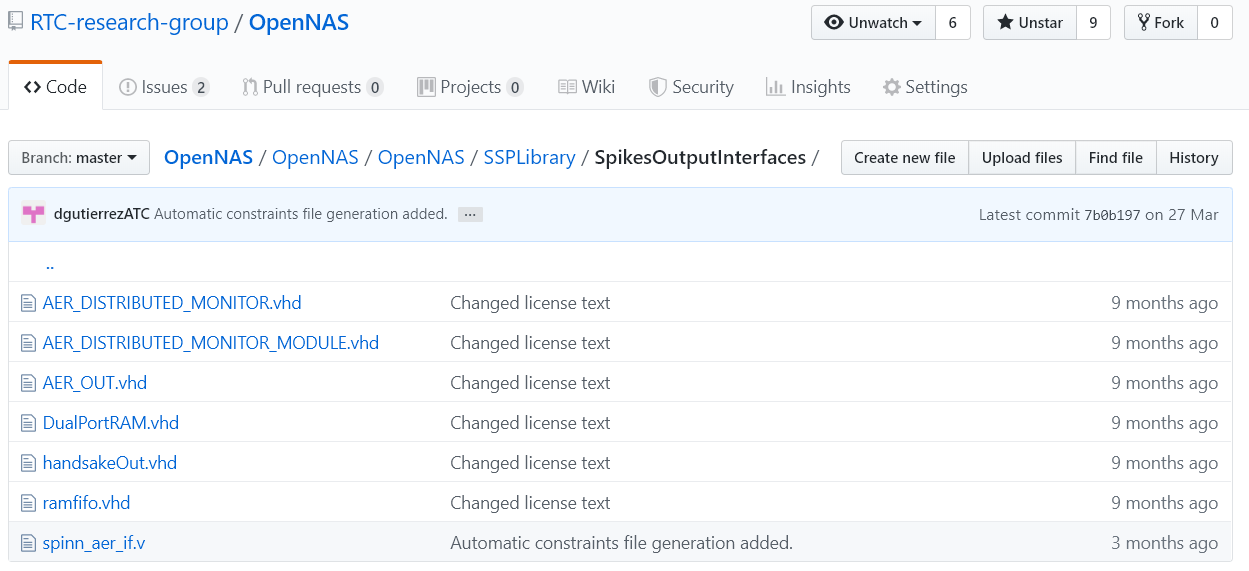
\includegraphics[width=1\textwidth]{images/Img09_SpikesOutputInterfaces.PNG}
\caption{\label{fig:OpenNAS_SpikeOutputInterface}NAS output interfaces VHDL modules.}
\end{figure}

%----------------------------------------------------------------------------------------
%	VisualStudio project
%----------------------------------------------------------------------------------------

\subsection{Running the VS application}

After to either download or clone the repository, it is time to run the OpenNAS application. The first step is to unzip the project. You will have into the new folder something like this:

\begin{figure}[H]
\centering
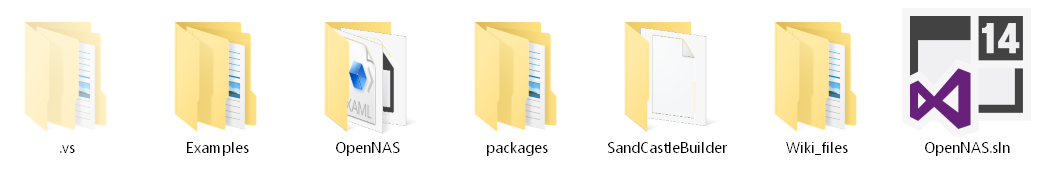
\includegraphics[width=0.5\textwidth]{images/Img10_OpenNAS_project.PNG}
\caption{\label{fig:OpenNAS_unziped_project}OpenNAS C\# project files.}
\end{figure}

For running the software, you first need to open the OpenNAS solution (OpenNAS.sln), and then the VisualStudio environment will be launched. If it is the first time that you open the solution, an advertisement message should appear. Don't worry about that, it is just a warning message about malicious code.

\begin{figure}[H]
\centering
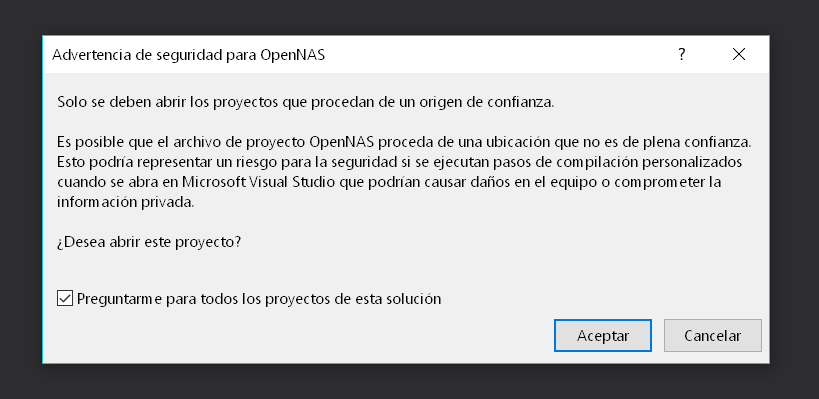
\includegraphics[width=0.9\textwidth]{images/Img11_VS_Advertencia_Seguridad.PNG}
\caption{\label{fig:VS_advertisement}Advertisement launched by the VisualStudio software the first time you open the OpenNAS project.}
\end{figure}

Click on "Accept", and the main window project will appear. The user can change the appearance of the OpenNAS tool, but never should change the controls, because the application will not work.

\begin{figure}[H]
\centering
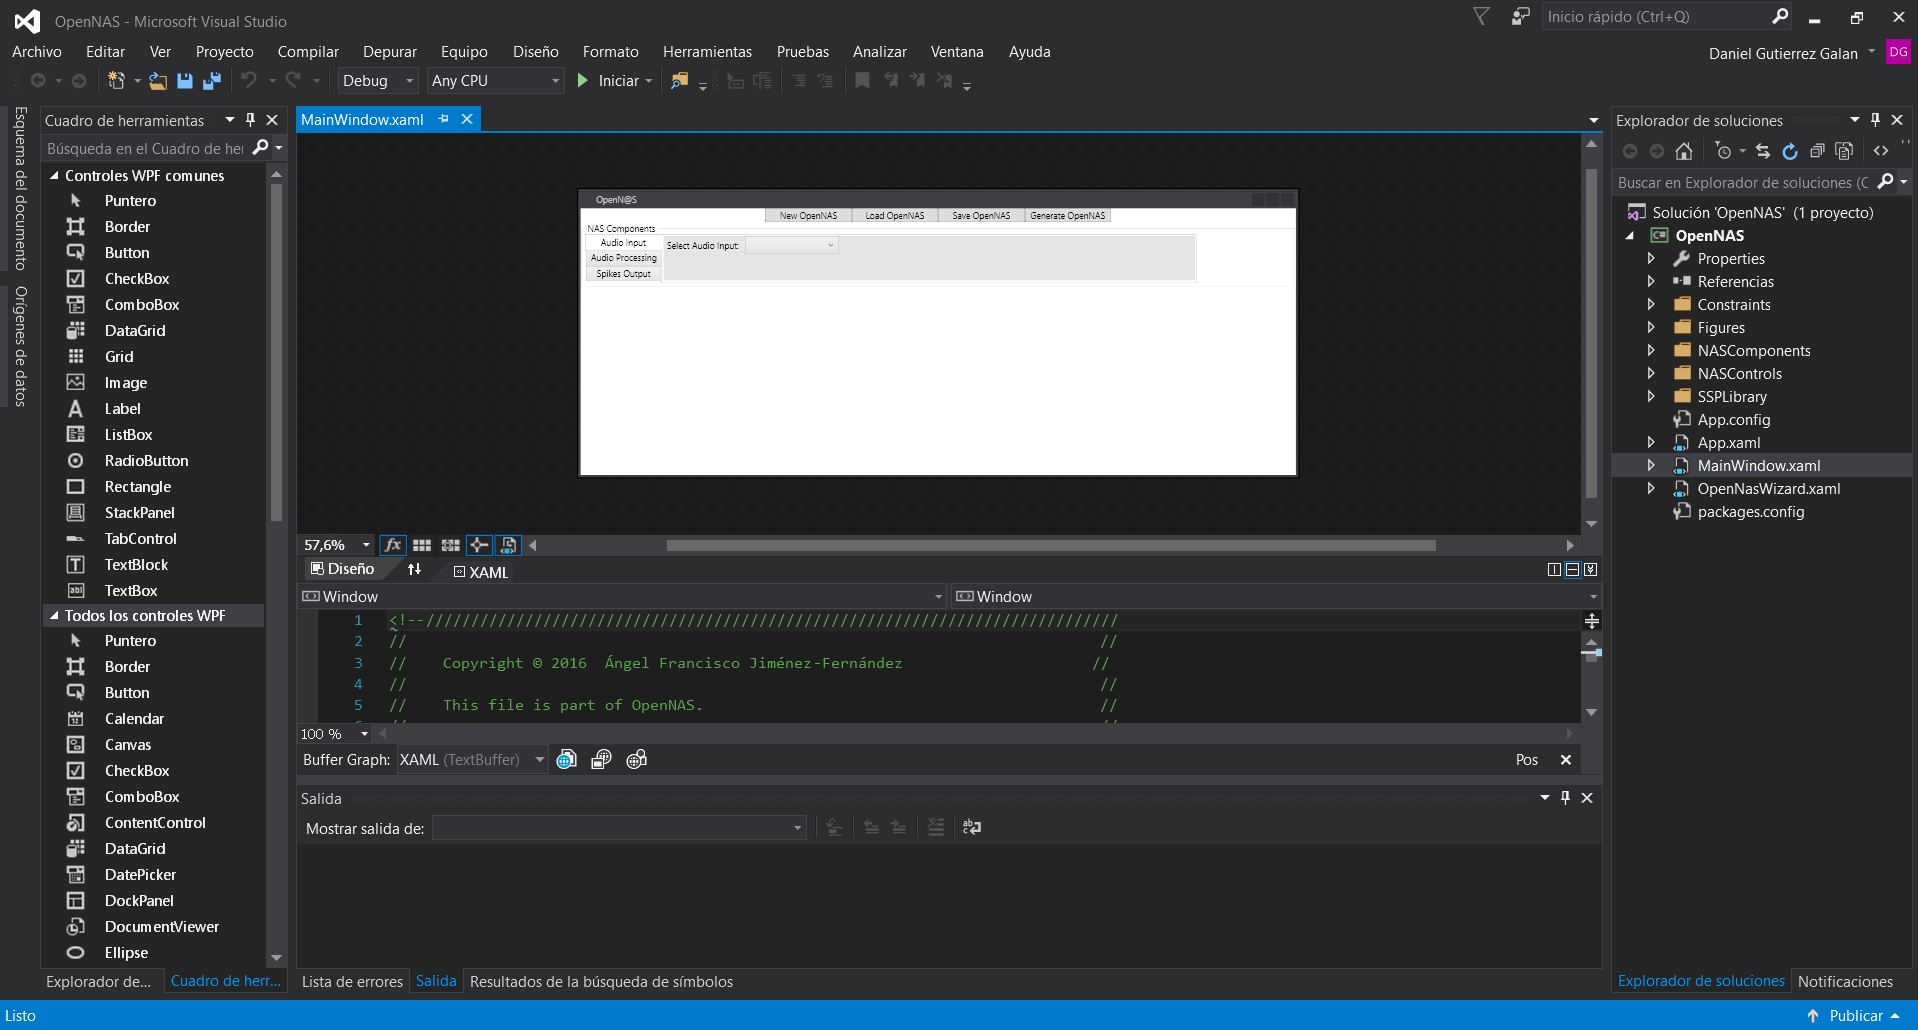
\includegraphics[width=1\textwidth]{images/Img12_VS_Proyecto.PNG}
\caption{\label{fig:VS_project}General view of the VisualStudio interface after open the OpenNAS project.}
\end{figure}

Now, the most difficult part: click on the "Start" button. A new window like the next one must appear...

\begin{figure}[H]
\centering
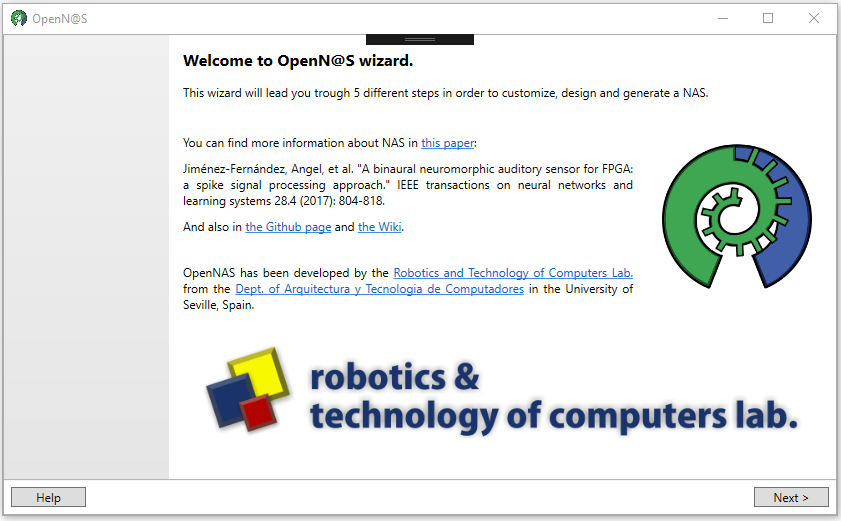
\includegraphics[width=1\textwidth]{images/Img13_VS_Init_App.PNG}
\caption{\label{fig:OpenNAS_Wizard_Welcome}OpenNAS wizard main window.}
\end{figure}

\textbf{CONGRATULATIONS}, OpenNAS is now running! That is the main window of the wizard. It just has one button to go forward to the wizard. Click on "Next" button to watch the next step of the NAS generation wizard.

In the step 1, users can select the NAS common settings, as the FPGA-based board in which the NAS will be loaded. NAS type (mono or stereo) and the numbers of channels can be set too. Be careful with the last field, the clock frequency. It will be used to set the spike-based processing blocks parameters correctly. By default, each board set this field automatically according with the board clock (except if you choose "Others"). However, if you want use another clock configuration, you can change the clock value. \textbf{Make sure you also implement this change in the VHDL files and ISE project!}

\begin{figure}[H]
\centering
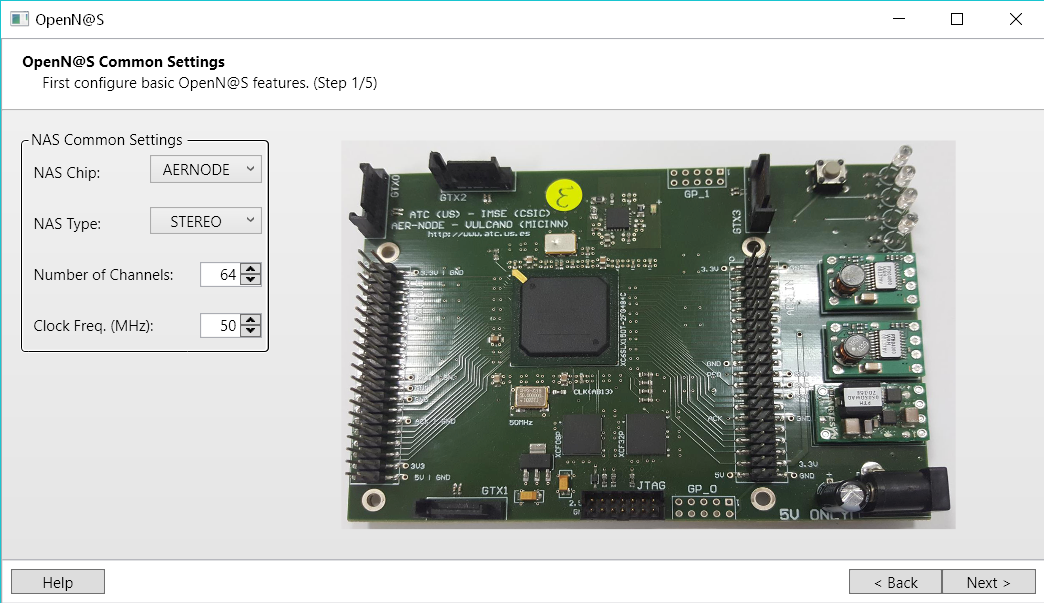
\includegraphics[width=1\textwidth]{images/Img14_VS_Step1.PNG}
\caption{\label{fig:OpenNAS_common_settings}First step of OpenNAS wizard. In this step, NAS common settings can be changed.}
\end{figure}

Here there is another option of board where NAS has been tested. If we check the clock frequency, its value has been set to 100 MHz.

\begin{figure}[H]
\centering
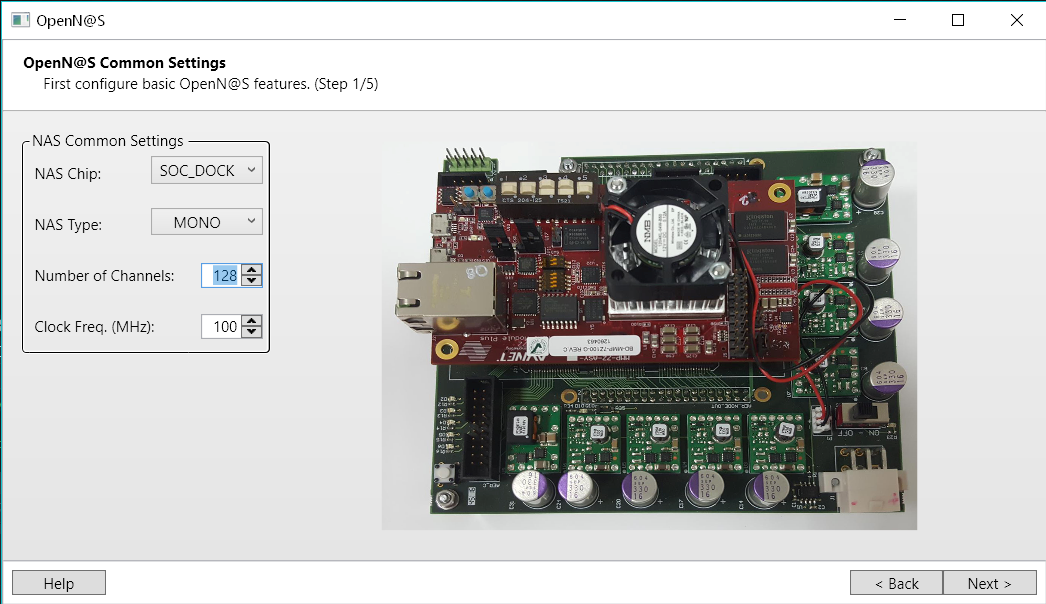
\includegraphics[width=1\textwidth]{images/Img15_VS_Step1_bis.PNG}
\caption{\label{fig:OpenNAS_s1}Setting the NAS chip to SOC\_DOCK board.}
\end{figure}

After the target board has been selected, and the common settings has been set according to your needs, it is time to select which audio input we will use. Clicking on "Next" button, we will go to the second step of the NAS wizard.

AC'97 audio codec is selected by default. Although it is not used in the AER-Node board, it was the first audio input device used by other Xilinx FPGA-based board. This option let you only to modify the spikes generation module clock divisor.

\begin{figure}[H]
\centering
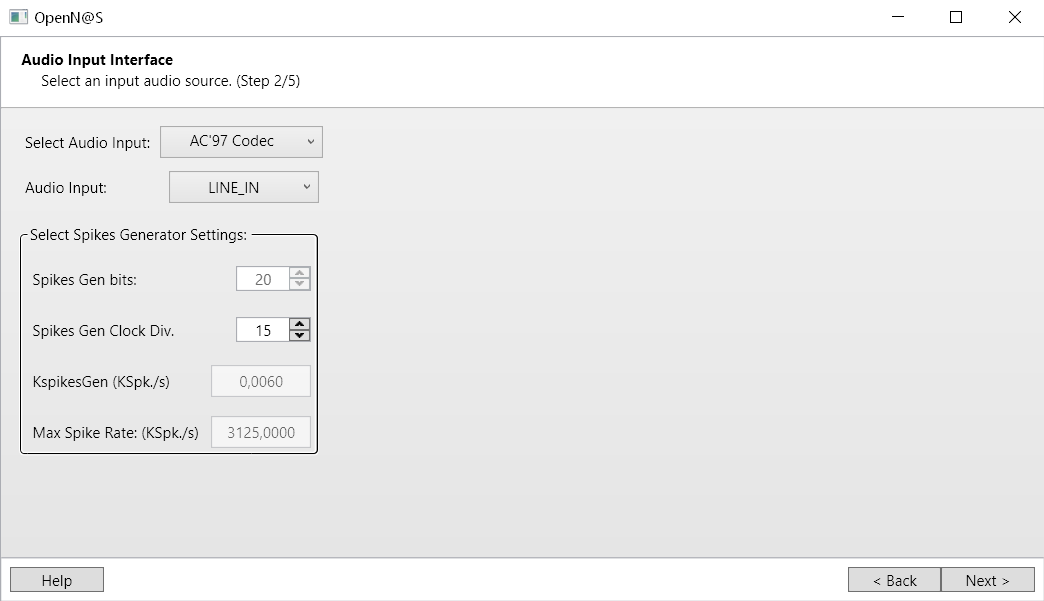
\includegraphics[width=1\textwidth]{images/Img16_S2_SelectInput.PNG}
\caption{\label{fig:OpenNAS_s2_ac97}Audio input from AC'97 audio codec.}
\end{figure}

There exist a new version of audio input interface. It consists in a PCB which has a pair of PDM microphones and also a new ADC for audio signals. This PCB was designed to be used along with the AER-Node board. Then, if you decided to use AER-Node board, you will be able to use the audio codec. This option is called "I2S" because the codec use that communication protocol to transfer the data.

\begin{figure}[H]
\centering
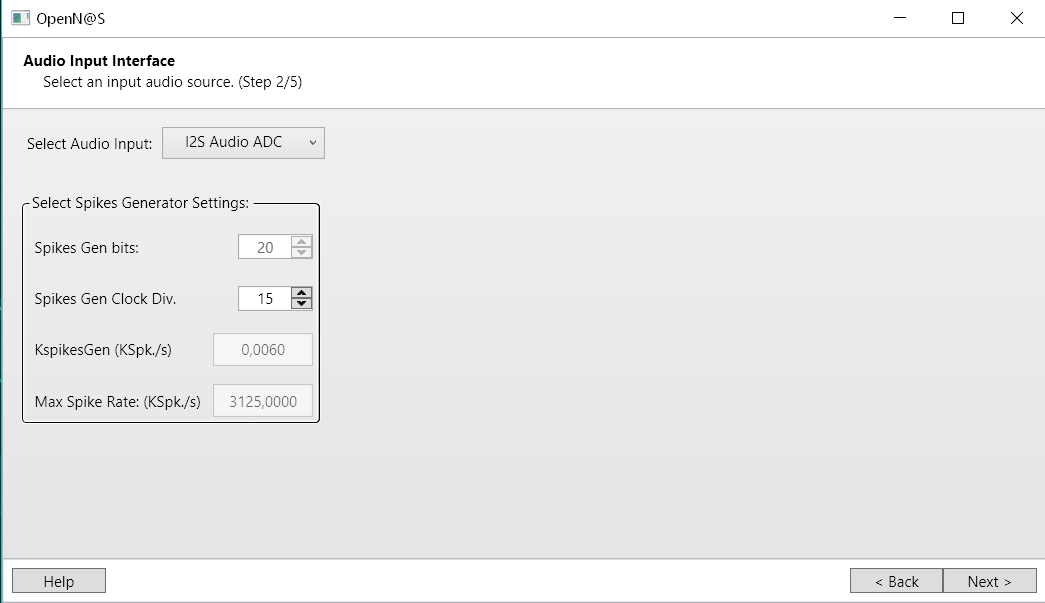
\includegraphics[width=1\textwidth]{images/Img17_S2_SelectInput_2.PNG}
\caption{\label{fig:OpenNAS_s2_i2s}Audio input from line-in connector.}
\end{figure}

Also, as we mentioned before, you can select to use the PDM microphones. User can set a lot of parameters, since it was implemented a FPGA module to convert the microphones output to spikes using several spike-based high/low pass filters.

\begin{figure}[H]
\centering
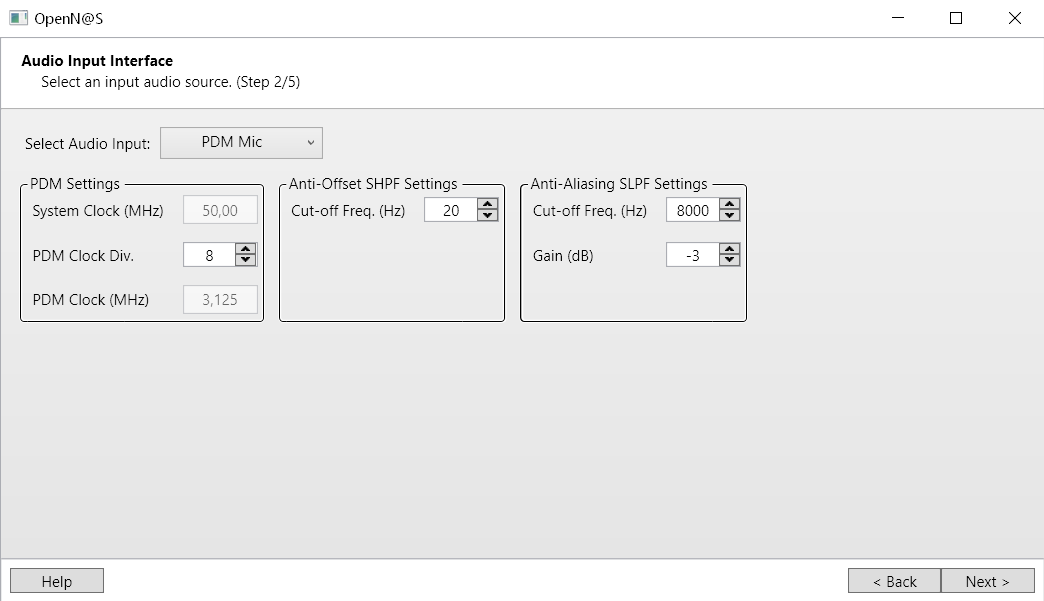
\includegraphics[width=1\textwidth]{images/Img18_S2_SelectInput_3.PNG}
\caption{\label{fig:OpenNAS_s2_pdm}Audio input from PDM microphones.}
\end{figure}

Thus the audio input interface board implements two different sound input devices, and the process of programming file is quiet long, the tool offers you the possibility of select both inputs, and to select which one would you use by using a jumper placed on the PCB.

\begin{figure}[H]
\centering
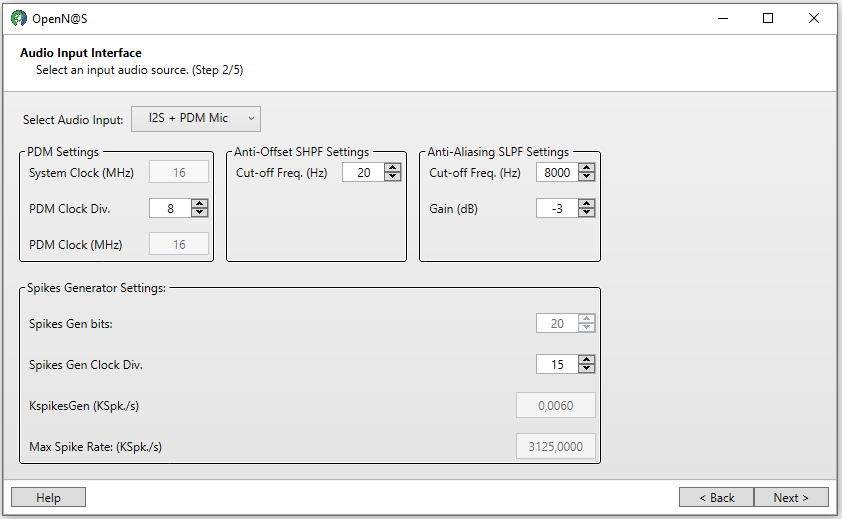
\includegraphics[width=1\textwidth]{images/Img19_S2_SelectInput_4.PNG}
\caption{\label{fig:OpenNAS_s2_i2s_pdm}Audio input from either line-in connector or PDM microphones, selected by a jumper position.}
\end{figure}

Now, let's begin to configure the most important part of the NAS model. The original NAS's filters architecture is in cascade, according to the biology. So, by default this option is selected. Yo can establish a frequency range, which is defined by default with the human audible sound range (from 20 Hz to 22 KHz). A critical parameter is the SBPF Output Att. (dB), due to this parameter modify the filters output attenuation, that means it controls the amount of spikes that we will have in the NAS output. By decreasing the value, less spikes will be obtained at the output. Actually, we are working with values close to -30 dB. 

\begin{figure}[H]
\centering
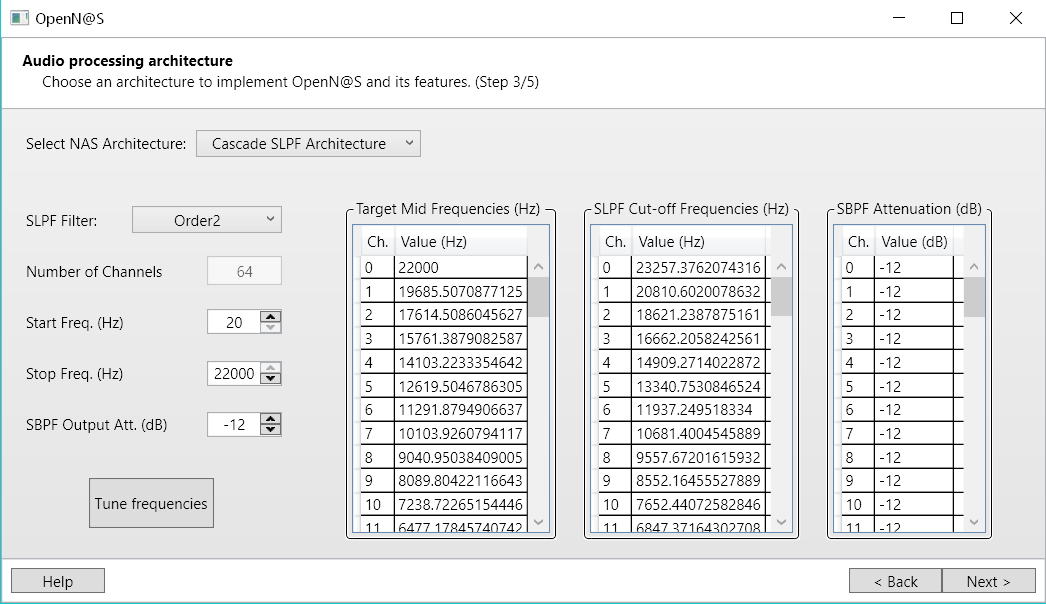
\includegraphics[width=1\textwidth]{images/Img20_S3_Arch.PNG}
\caption{\label{fig:OpenNAS_s3_cascade}Selecting the NAS architecture. Cascade architecture is mostly used, and it is by default in the OpenNAS.}
\end{figure}

Filter's channels frequencies are calculated automatically by the software based on the specified architecture by the user. However, if you modify the attenuation value, you need to click on "Tune frequencies" button to recalculated all the parameters.

There is another NAS architecture approach, the parallel filter bank architecture. The parallel architecture is still under develop, but if you are curious you can take a look and try to use it.

\begin{figure}[H]
\centering
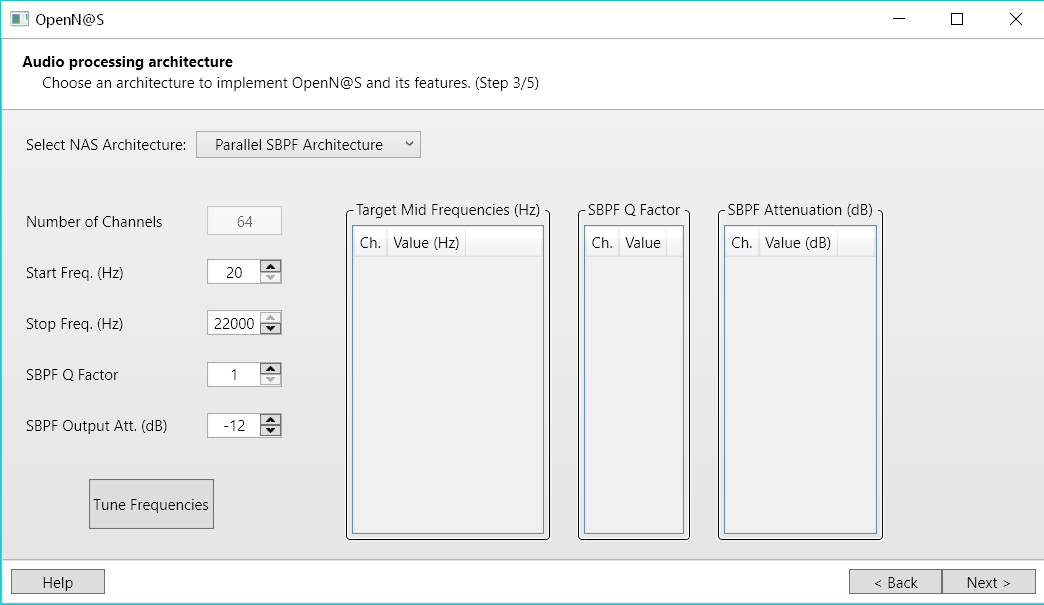
\includegraphics[width=1\textwidth]{images/Img21_S3_Arch_bis.PNG}
\caption{\label{fig:OpenNAS_s3_parallel}Parallel architecture open a different approach to the audio processing.}
\end{figure}

Almost the end, but not less important. It is time to choose the output interface. This step is completely dependent of what do you want to do by using the NAS. According with our experience, we recommend first to select the Spikes Distributed Monitor, which allows you to visualize the NAS output in real-time using the jAER software. Then, you can perform some recordings with your audio input dataset, and to analyze it by using the NAVIS tool, specifically designed and implemented for that purpose. NOTE: it is not recommendable to change the parameter values unless you need it.

\begin{figure}[H]
\centering
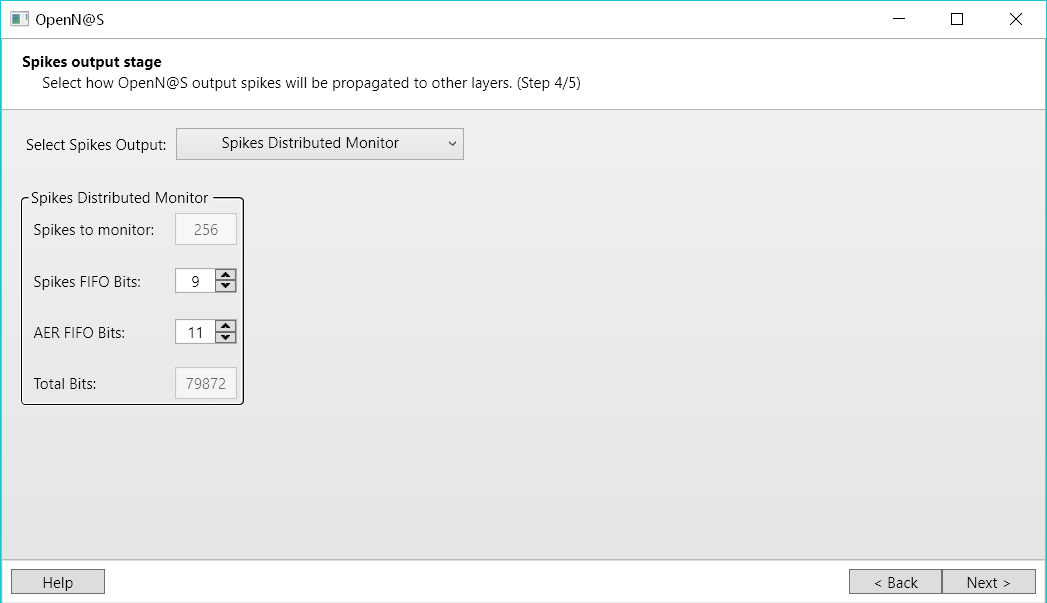
\includegraphics[width=1\textwidth]{images/Img22_S4_OutInterface.PNG}
\caption{\label{fig:OpenNAS_s4_monitor}Using the AER Distributed Monitor as output interface allow you to monitor the NAS output in real time..}
\end{figure}

After checking the NAS output, and to be sure that the output will be useful for you, OpenNAS allows you the possibility of to connect the NAS with the SpiNNaker machine (both 4-chips and 48-chips machines). There are two versions of the AER-SpiNNaker interface; the v1, which is able to send spikes from the NAS to the SpiNNaker machine through the SpiNNaker link (using an adapter board). Any parameters are not needed in this case.

\begin{figure}[H]
\centering
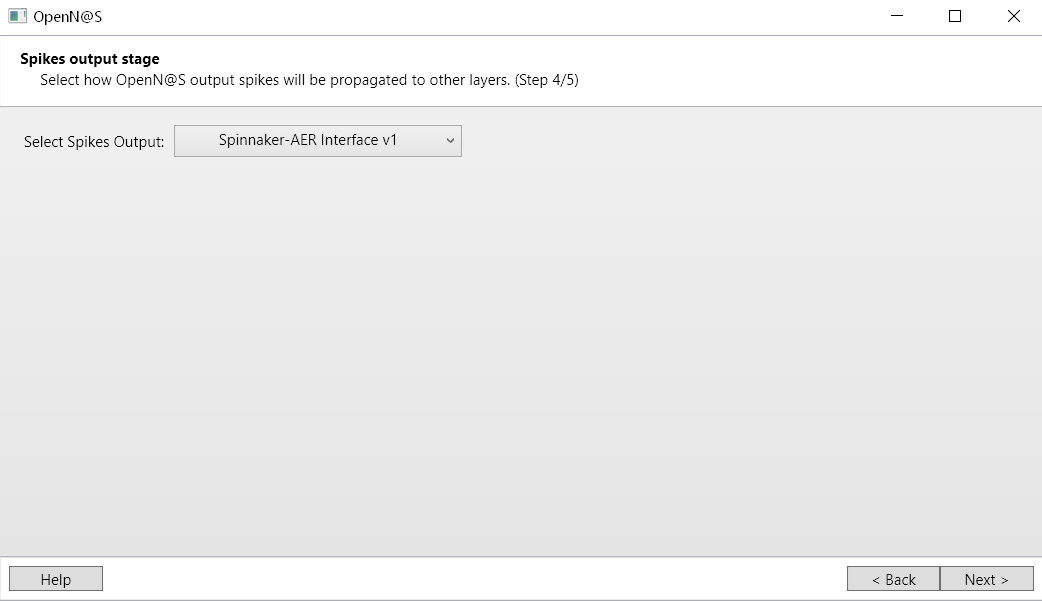
\includegraphics[width=1\textwidth]{images/Img23_S4_OutInterface_2.PNG}
\caption{\label{fig:OpenNAS_s4_spinnv1}With SpiNNaker interface v1 you can send AER events from the NAS to the SpiNNaker machine.}
\end{figure}

The second version of AER-SpiNNaker interface is an adaptation of the work performed by Luis Plana to connect AER devices with the SpiNNaker machine in real time allowing bi-directional communication. Here you are the \textcolor{blue}{\href{https://github.com/SpiNNakerManchester/spio}{GitHub link}} of the original repository. There is also a complete documentation which we used to modify the original version in \textcolor{blue}{\href{http://spinnakermanchester.github.io/docs/fpga_aer/}{this link}}.

And, why don we not have a mixed output between AER monitor and SpiNNaker? Of course, we have implemented a version in which you can monitor the NAS output that are being sending to the SpiNNaker machine using jAER. But it could be a problem, because for each output spike, you will need the ACK signal from both jAER application and SpiNNaker machine. Hence, the system could work slowly.

The last step, after spend like... 2 minutes setting the OpenNAS is to generate the NAS files according with your parameters. You need to specify a folder in which all the files will be copied.

\begin{figure}[H]
\centering
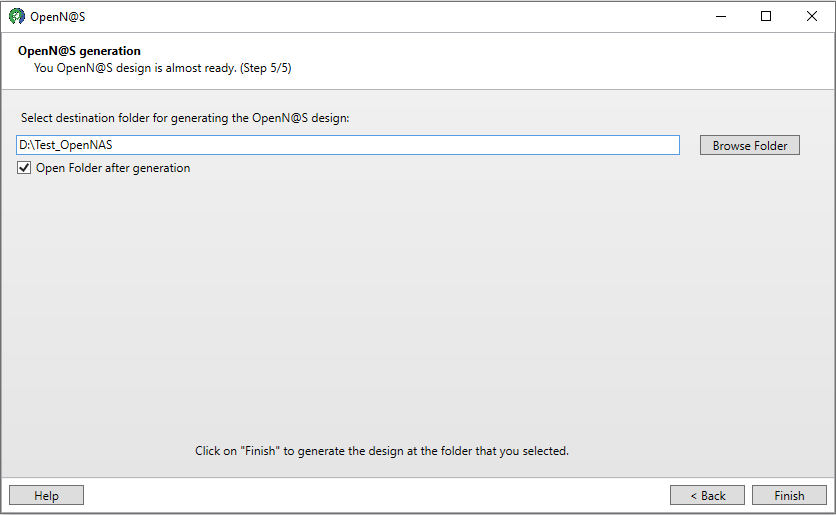
\includegraphics[width=1\textwidth]{images/Img24_S5_SaveFiles.PNG}
\caption{\label{fig:OpenNAS_s5_destination_folder}Select a destination folder to save the NAS files.}
\end{figure}

We recommend to create a very simple folders architecture: the main folder, named for example NAS\_PDM\_64ch\_MONO\_Monitor, and one folder to the source files, named "sources", and another one in which the ISE project will be created, named "project". Once the destination folder is selected, just click on the "Finish" button.

\begin{figure}[H]
\centering
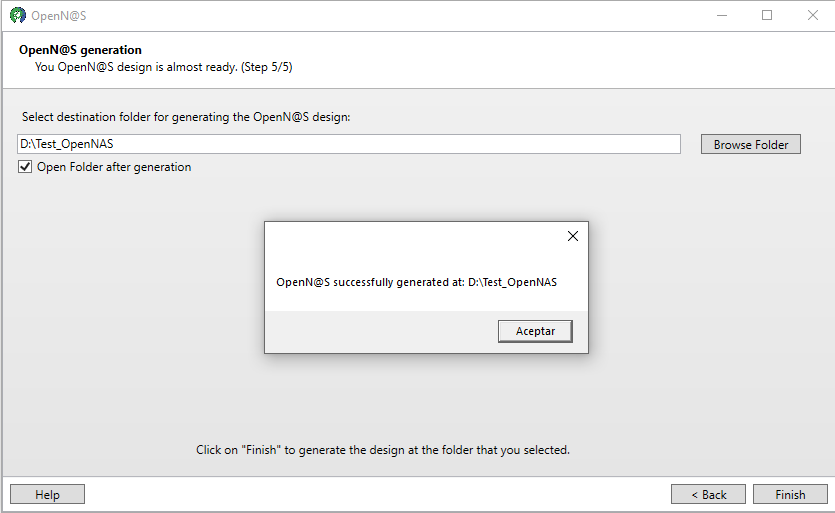
\includegraphics[width=1\textwidth]{images/Img25_S5_SaveFiles_OK.PNG}
\caption{\label{fig:OpenNAS_s5_success}Files were generated successfully.}
\end{figure}

If everything is OK, a message window should appear telling you "OpenNAS successfully generated" and also showing you the destination folder. At this point, NAS HDL files has been generated taking into account your preferences, and you can take a look of the source code.

Anadir vista de los archivos que genera y que son cada uno. Hablar del xml.



%----------------------------------------------------------------------------------------
%	ISE HDL project
%----------------------------------------------------------------------------------------

\subsection{Creating a Xilinx ISE project}

By now, a lot of things have been taking into account to generate correctly your NAS model. And in this moment, since we already have the NAS VHDL files, you can decide what will you do with those files. You could want just load the files into the FPGA, or maybe you need to add new VHDL modules or modify the NAS VHDL modules to test something... In any case, you will need to create a new ISE project to, finally, generate the programming file with .bit extension and then to program the FPGA.

If you have an AER-Node board, SOC\_DOCK board or ZTEX 2.13 board (OpalKelly will be available soon), and you do not want to add/change any VHDL modules, you can directly get the .bit file by running a .tcl script by using the ISE Design Suite 32 Bit Command Prompt. (Still under development, but it will be available soon!).

Meanwhile, of if you do not have one of those boards, you will need to create a ISE project manually, to configure it correctly and to add the source files by hand. First step, of course, is open the ISE 32-bit Project Navigator. The icon looks like is showed in the next Figure~\ref{fig:ISE_icon}:

\begin{figure}[H]
\centering
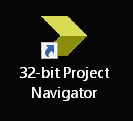
\includegraphics[width=0.3\textwidth]{images/Img26_FindISE.PNG}
\caption{\label{fig:ISE_icon}ISE Project Navigator icon.}
\end{figure}

Left click on the icon twice, and then the project navigator will be opened. Next image show us how the program looks like when it is started.

\begin{figure}[H]
\centering
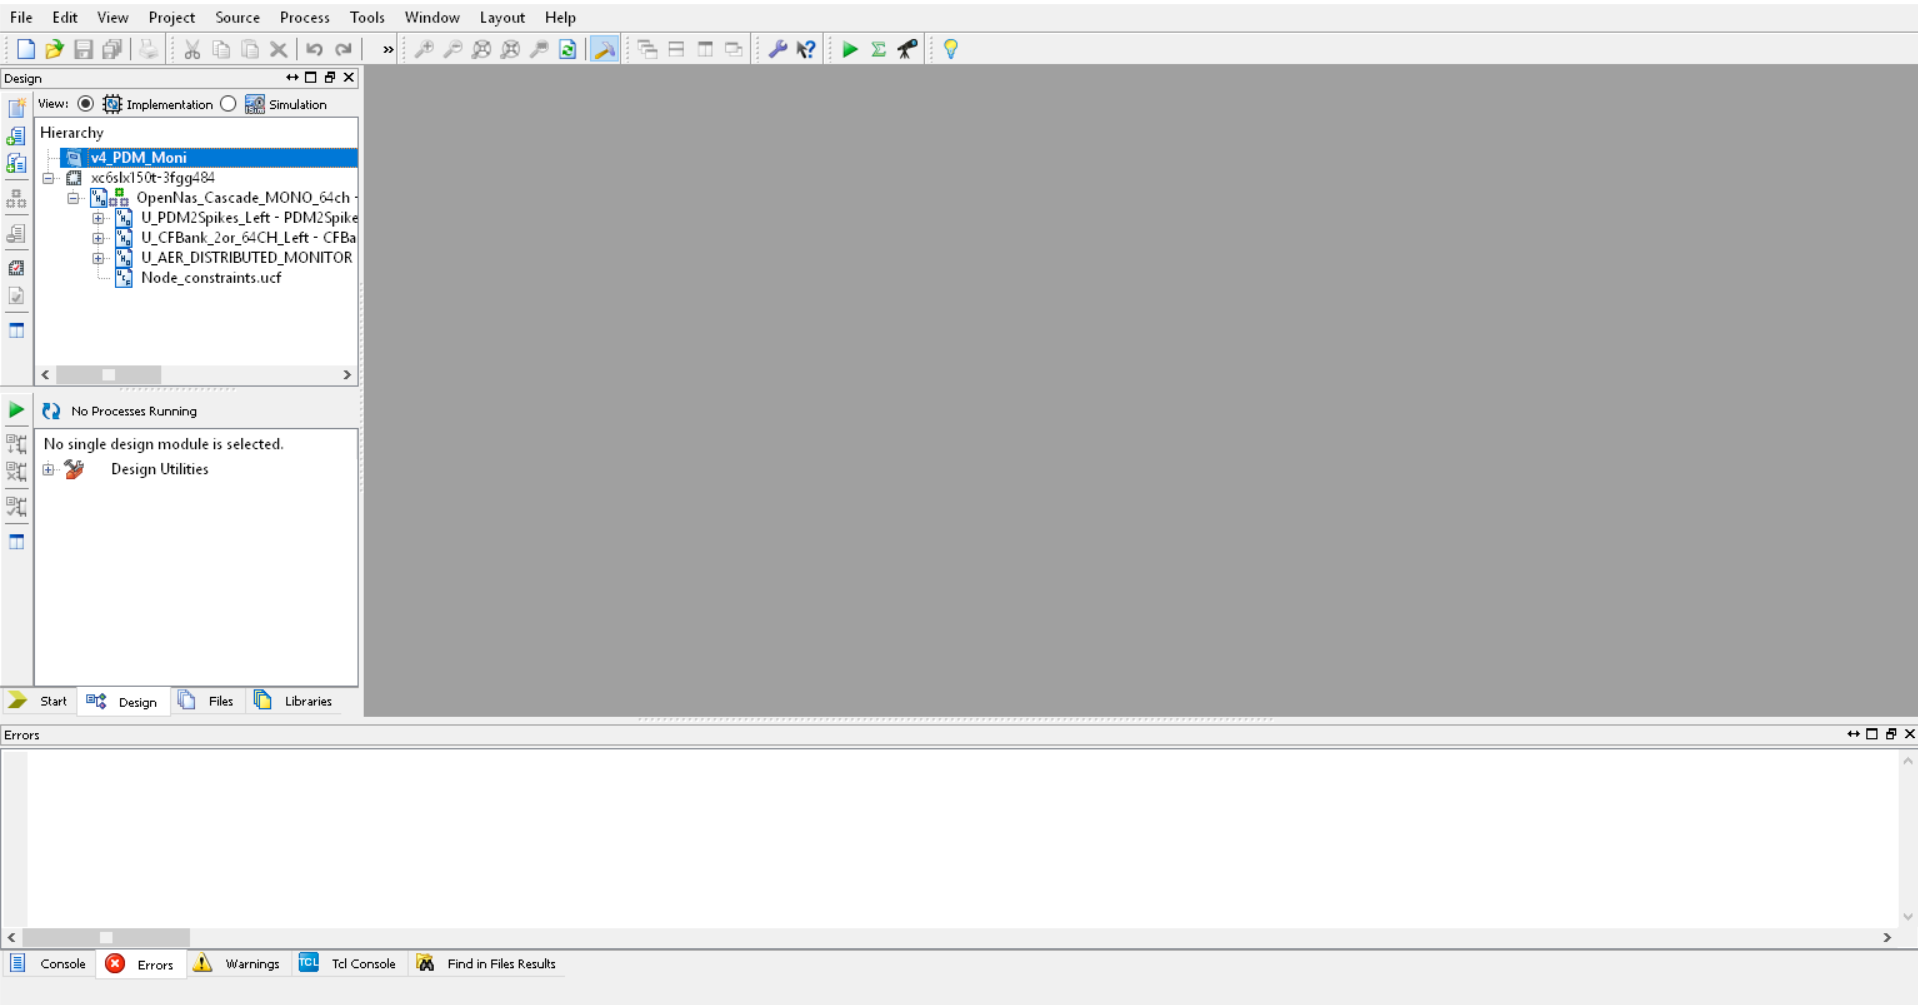
\includegraphics[width=1\textwidth]{images/Img27_ISE_Init.PNG}
\caption{\label{fig:ISE_main_windows}ISE Project Navigator main view.}
\end{figure}

So, we need first to create a new project. To do that, go to File, and select New Project.

\begin{figure}[H]
\centering
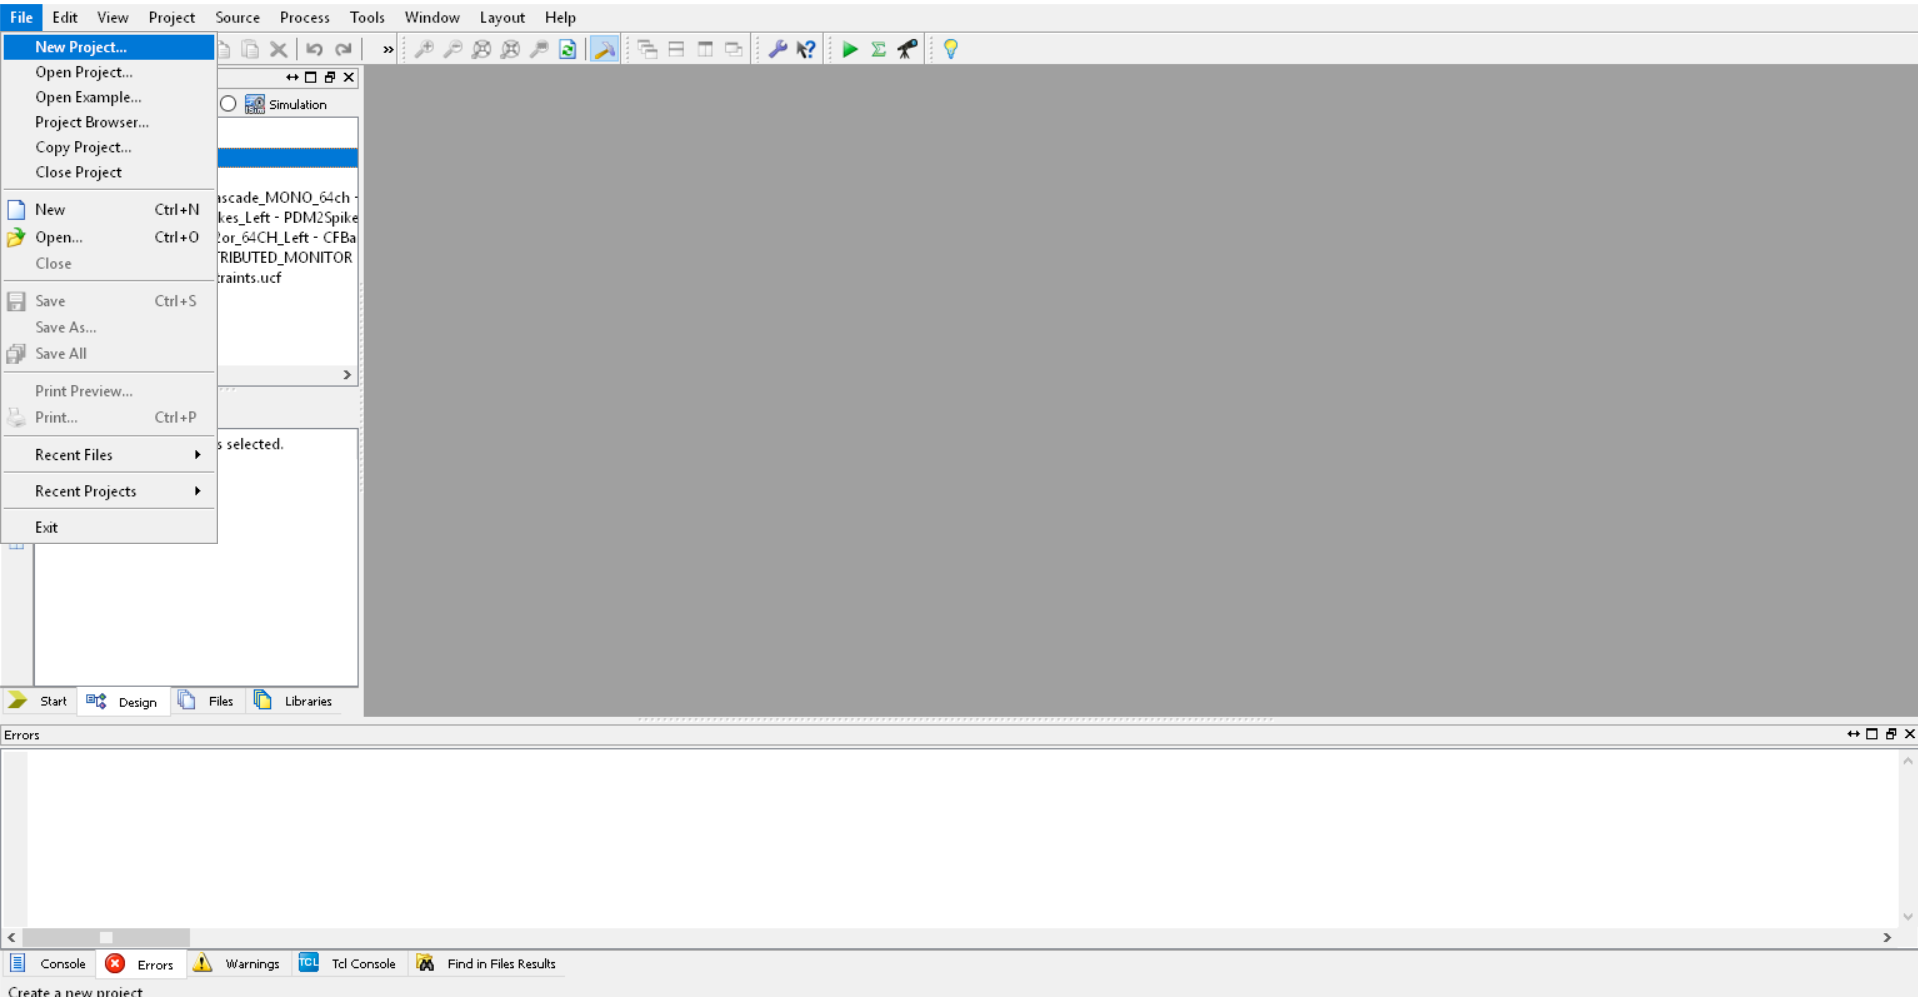
\includegraphics[width=1\textwidth]{images/Img28_File_NewProject.PNG}
\caption{\label{fig:ISE_create_project}Creating a new project in ISE Project Navigator.}
\end{figure}

Then a new window appear. This is the New Project Wizard, and it is easy to follow. Let's start it.

\begin{figure}[H]
\centering
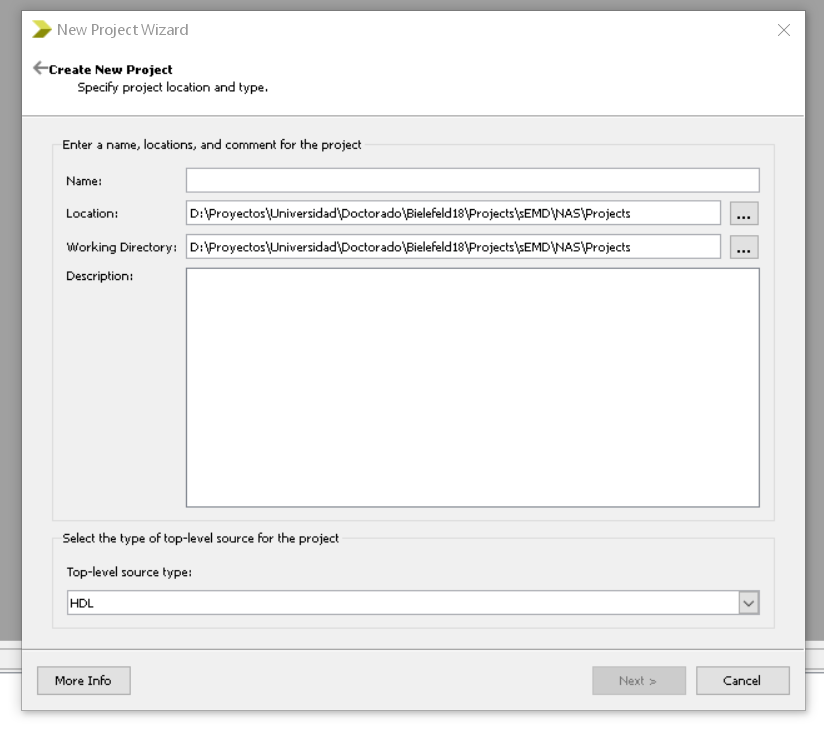
\includegraphics[width=1\textwidth]{images/Img29_NewProject_Wizard.PNG}
\caption{\label{fig:ISE_project_wizard}ISE new project wizard.}
\end{figure}

Like in every new project, you have to indicate the project name. According to the folders architecture aforementioned, we recommend to select the same name used by the sources folder. In our case, our project will be named NAS\_PDM\_64ch\_MONO\_Monitor. And the location will be ../NAS\_PDM\_64ch\_MONO\_Monitor/project/. Now, click on the "Next" button.

\begin{figure}[H]
\centering
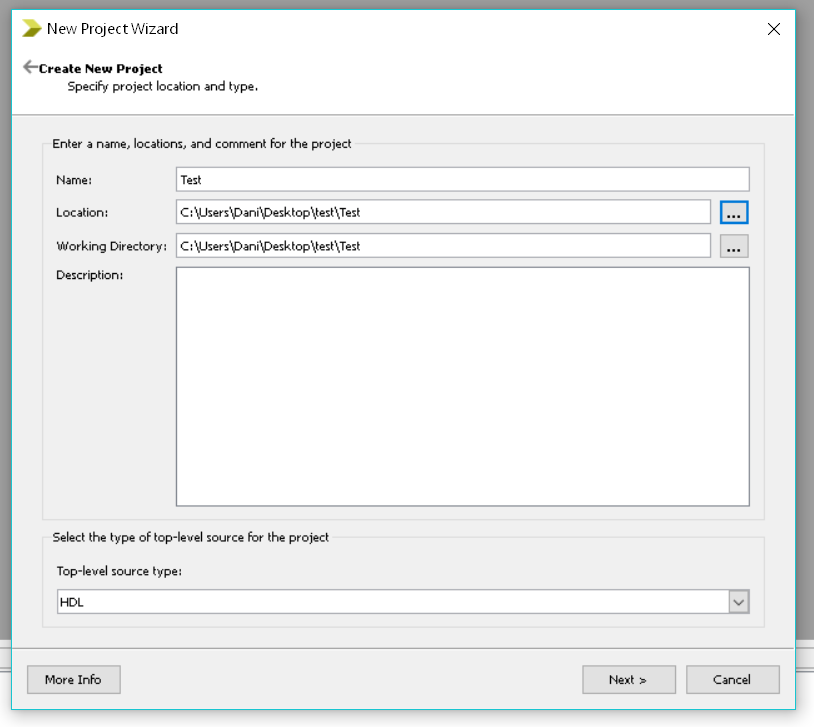
\includegraphics[width=1\textwidth]{images/Img30_NewProject_Wizard_bis.PNG}
\caption{\label{fig:ISE_name_location_project}Setting the ISE project name and the project localization.}
\end{figure}

\textbf{CAUTION!} This step should be done carefully. In the project settings step, the FPGA chip must be selected. Make sure that all the fields have the same values that the showed in the image. Those values are only valid if the AER-Node board is used. For others board, user should make its own project settings. 

\begin{figure}[H]
\centering
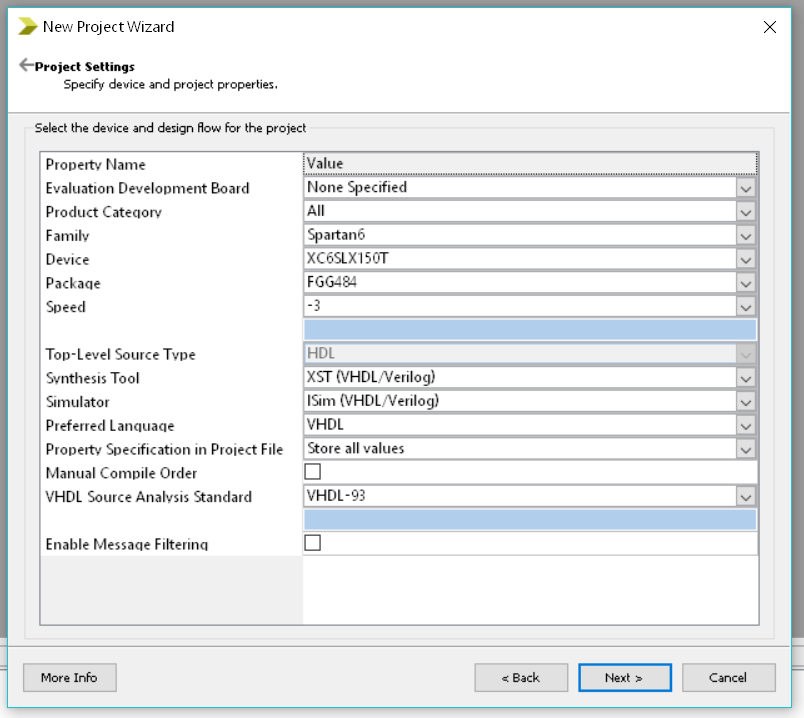
\includegraphics[width=1\textwidth]{images/Img31_NewProject_FPGA_conf.PNG}
\caption{\label{fig:ISE_project_settings}Correct project settings to create a ISE project for the AER-Node board.}
\end{figure}

At the end of the wizard, a summary of the new project is showed. Check this summary to prevent future errors. If everything is correct, click on "Finish".

\begin{figure}[H]
\centering
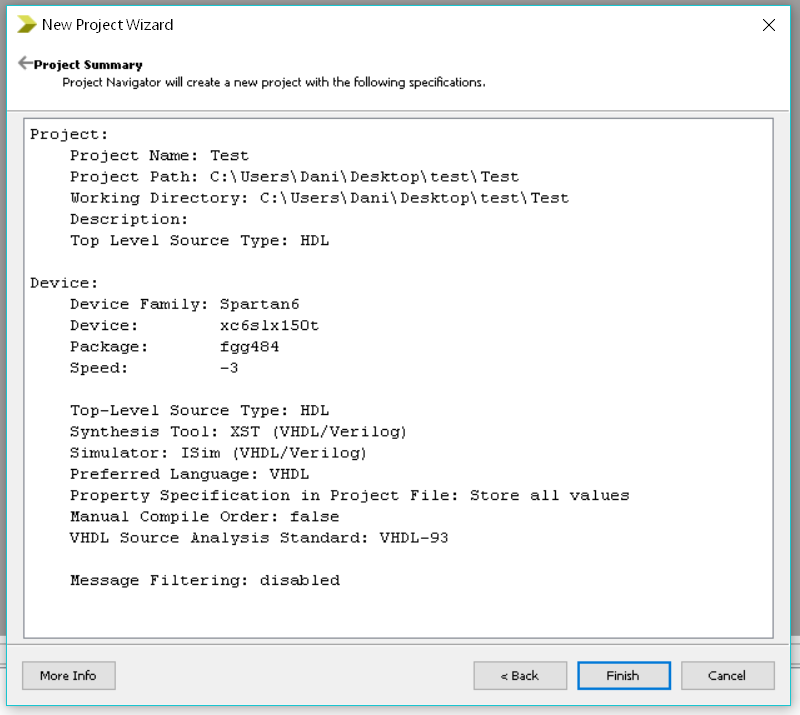
\includegraphics[width=1\textwidth]{images/Img32_NewProject_Summary.PNG}
\caption{\label{fig:ISE_project_summary}ISE project settings summary.}
\end{figure}

Our project is now created, and we can see in the top left a new folder with the name of our project, and the selected FPGA chip.

\begin{figure}[H]
\centering
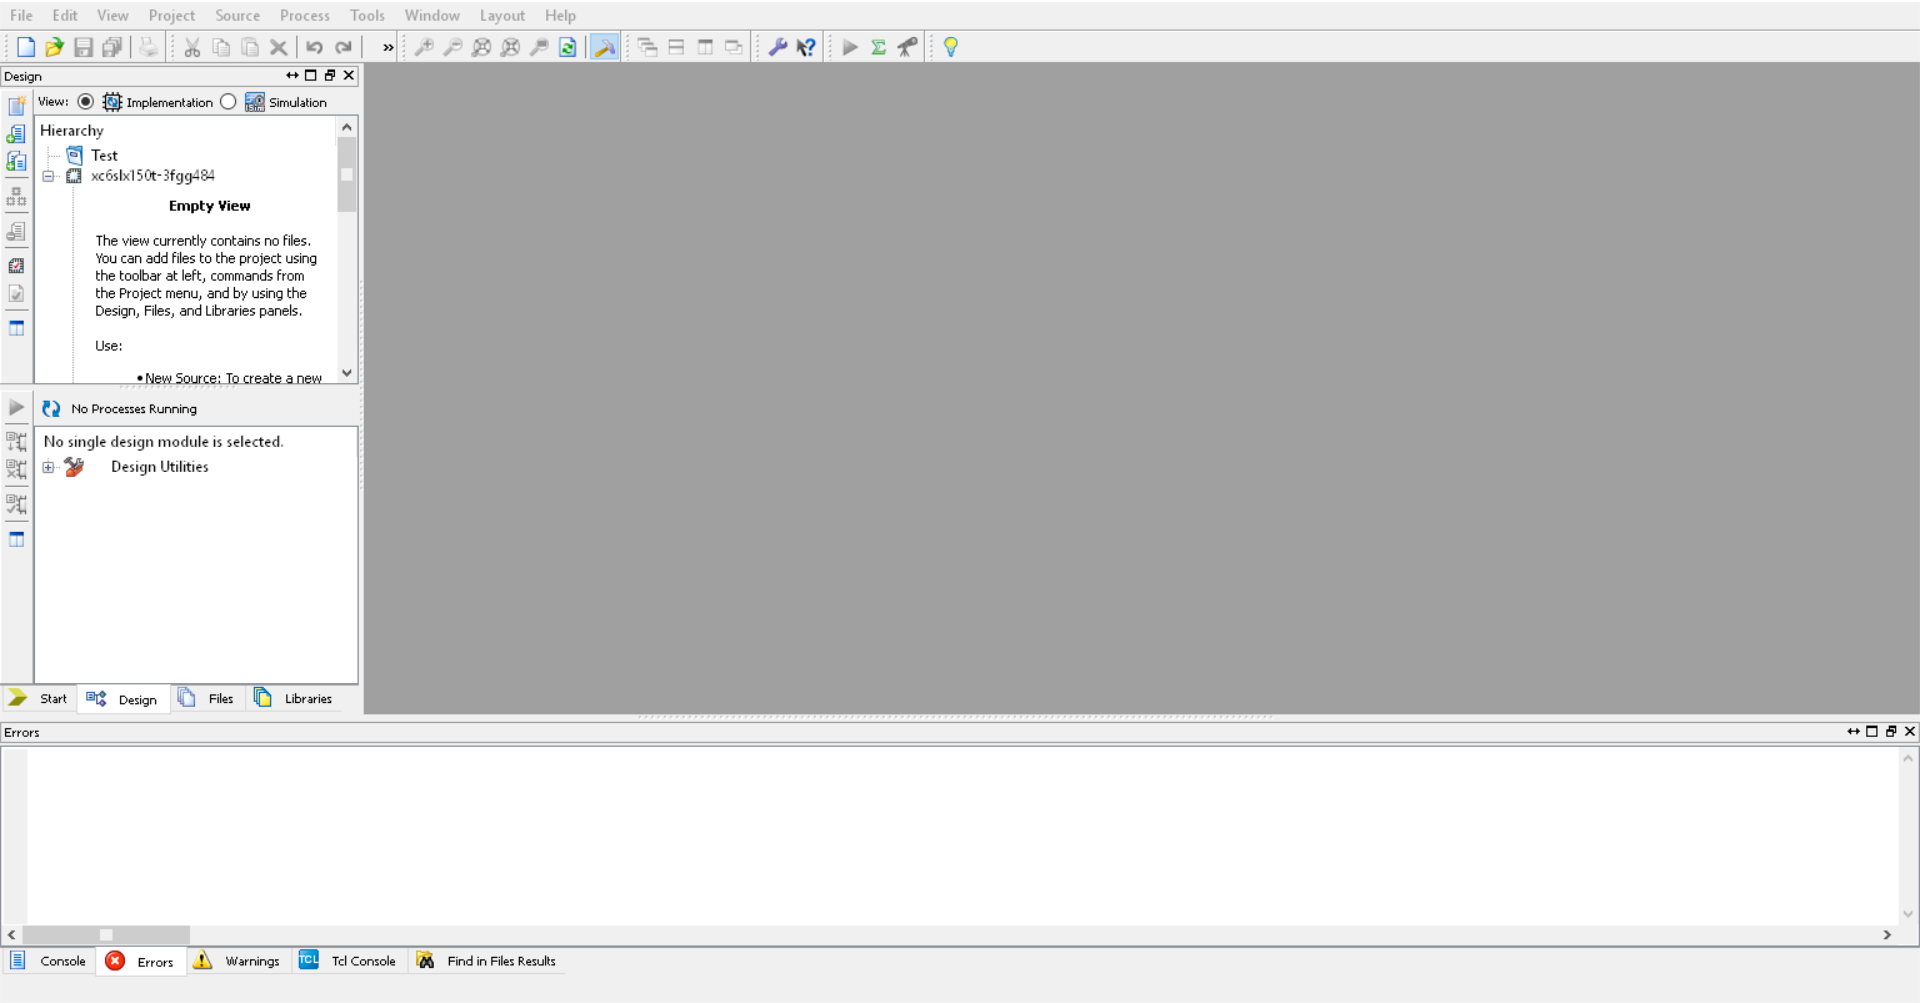
\includegraphics[width=1\textwidth]{images/Img33_NewProject.PNG}
\caption{\label{fig:ISE_project_created}Main view after create a new project.}
\end{figure}

And now, the last "very important" step, which is to add the NAS VHDL files generated by the OpenNAS into the new ISE project. But, why is this an important step? There are many reasons, but the two more important reasons are: because you need to add the correct files, and because is recommendable to add those files, not to add a copy of those files. Let see. First, make right click either on the project folder or on the selected chip. A menu appears, and then select "Add sources".

\begin{figure}[H]
\centering
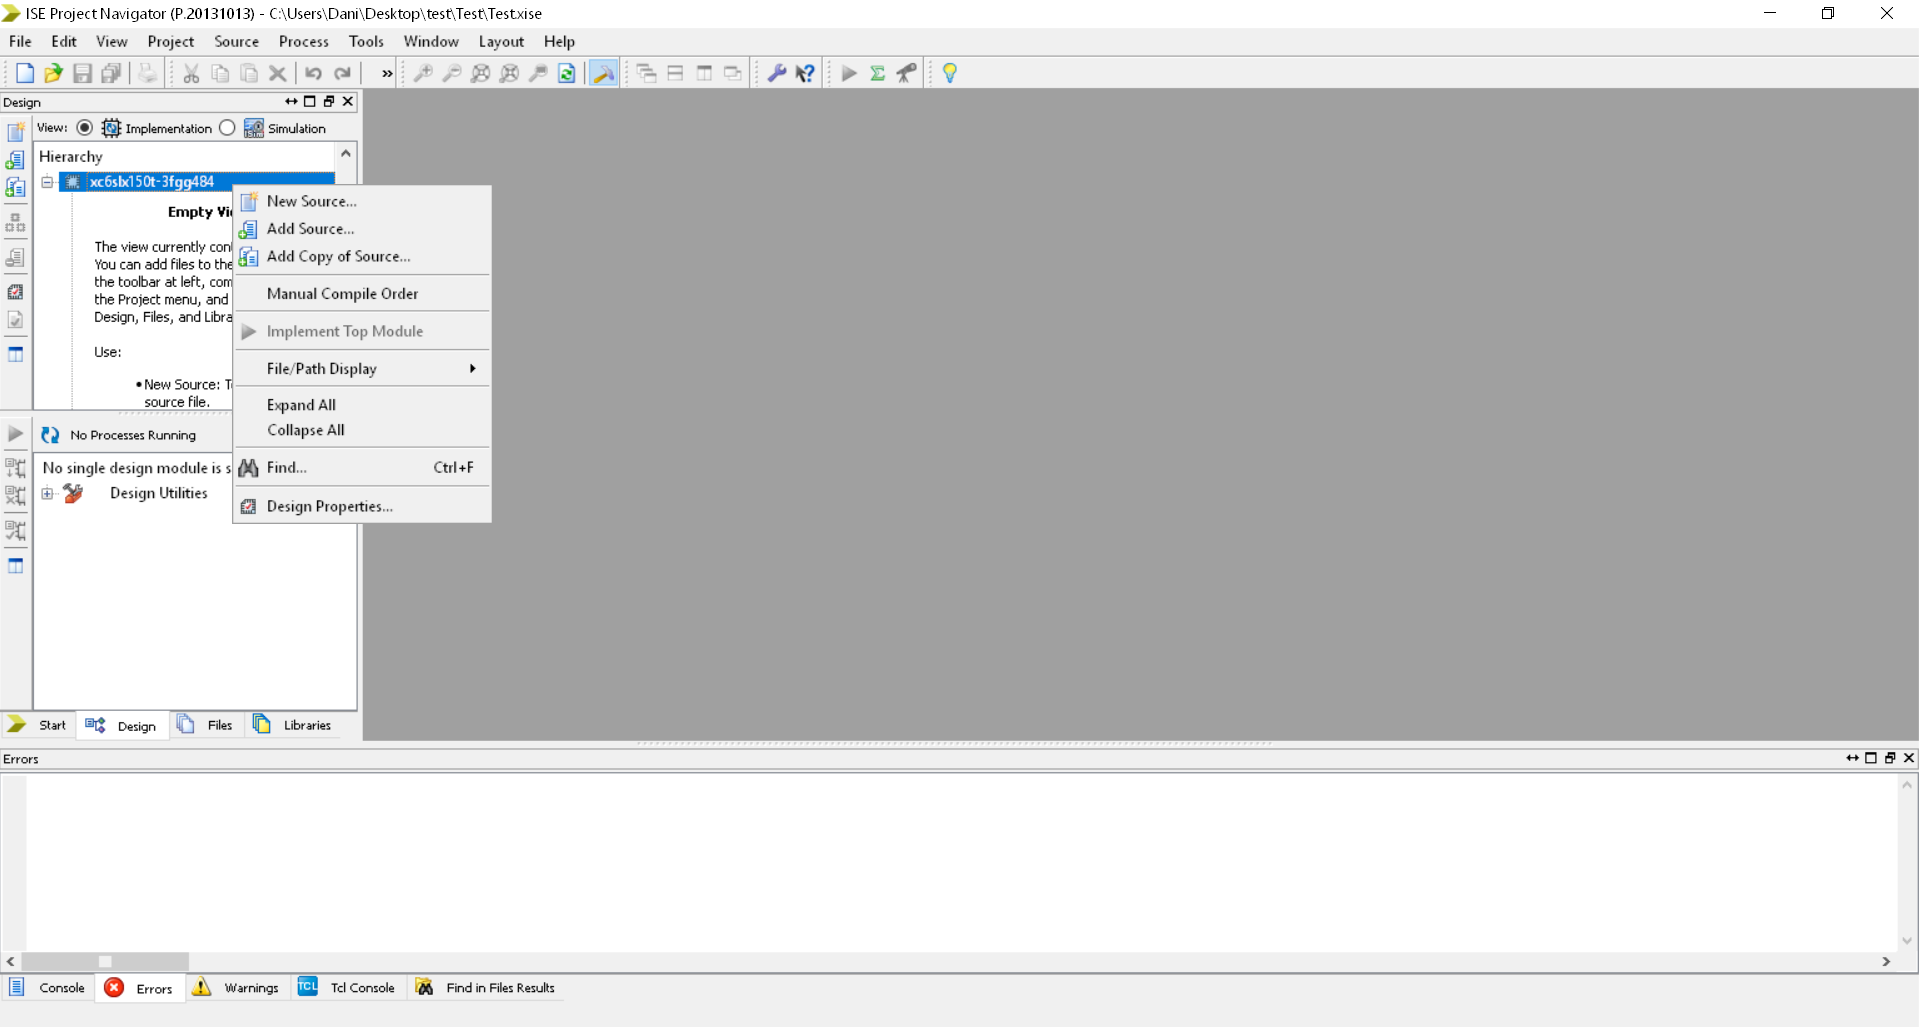
\includegraphics[width=1\textwidth]{images/Img34_AddSource.PNG}
\caption{\label{fig:ISE_add_sources}Ready for adding the NAS VHDL sources.}
\end{figure}

An emergent windows should appear to navigate where the NAS VHDL sources are. But be careful, if it is not the first project that you have created, then you may select the wrong OpenNAS sources with different parameters. If you follow our recommendation of how to organize the NAS projects, the source files should be in ../NAS\_PDM\_64ch\_MONO\_Monitor/sources/.

\begin{figure}[H]
\centering
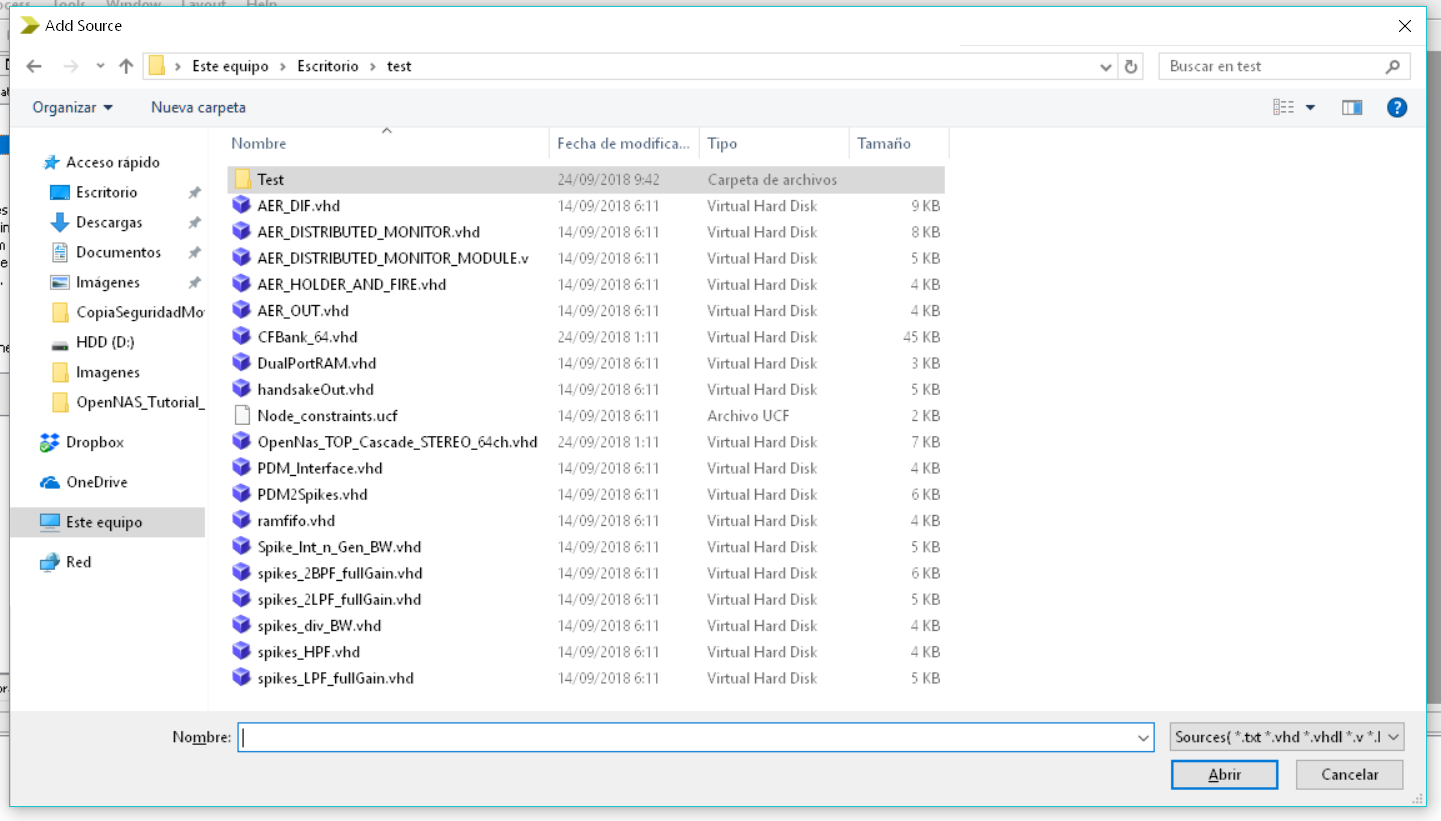
\includegraphics[width=1\textwidth]{images/Img35_SelectFiles.PNG}
\caption{\label{fig:ISE_look_for_sources}Go to the destination folder in which the NAS VHDL were saved.}
\end{figure}

When there, just select all the files, and click on "Open" button to add them.

\begin{figure}[H]
\centering
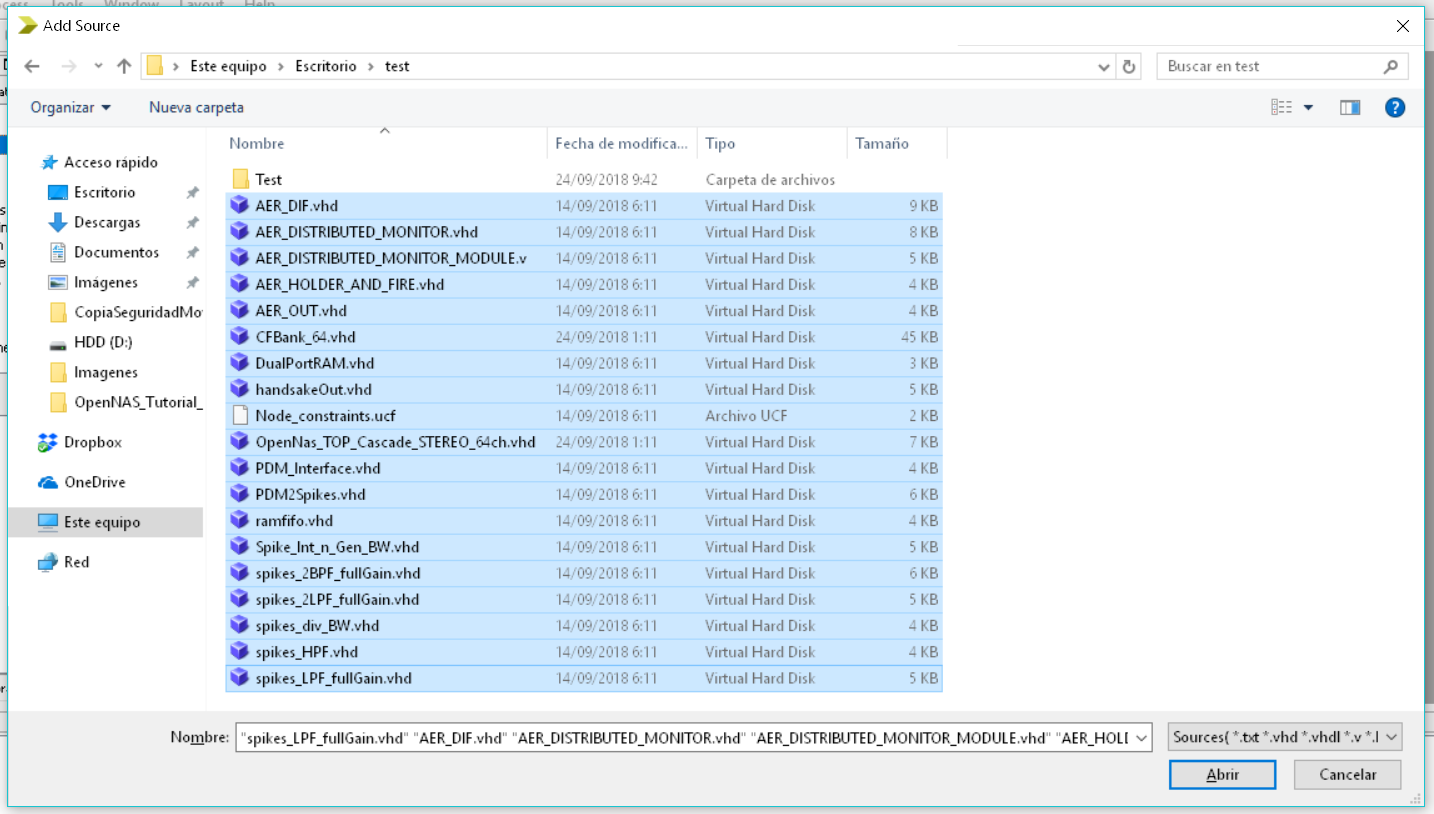
\includegraphics[width=1\textwidth]{images/Img36_SelectFiles_bis.PNG}
\caption{\label{fig:ISE_select_all}Select all the files, except the .xml file.}
\end{figure}

In a ISE project, source files can be included for simulation, for implementation, or for all. If we take a look, by default all files have the field "Association" to "All" except the constraint file .ucf, which does not make sense in a simulation process. We do not need change any values. But if you want to add a testbench file, the file association should be "Simulation". Click on "OK" to finish this step.

\begin{figure}[H]
\centering
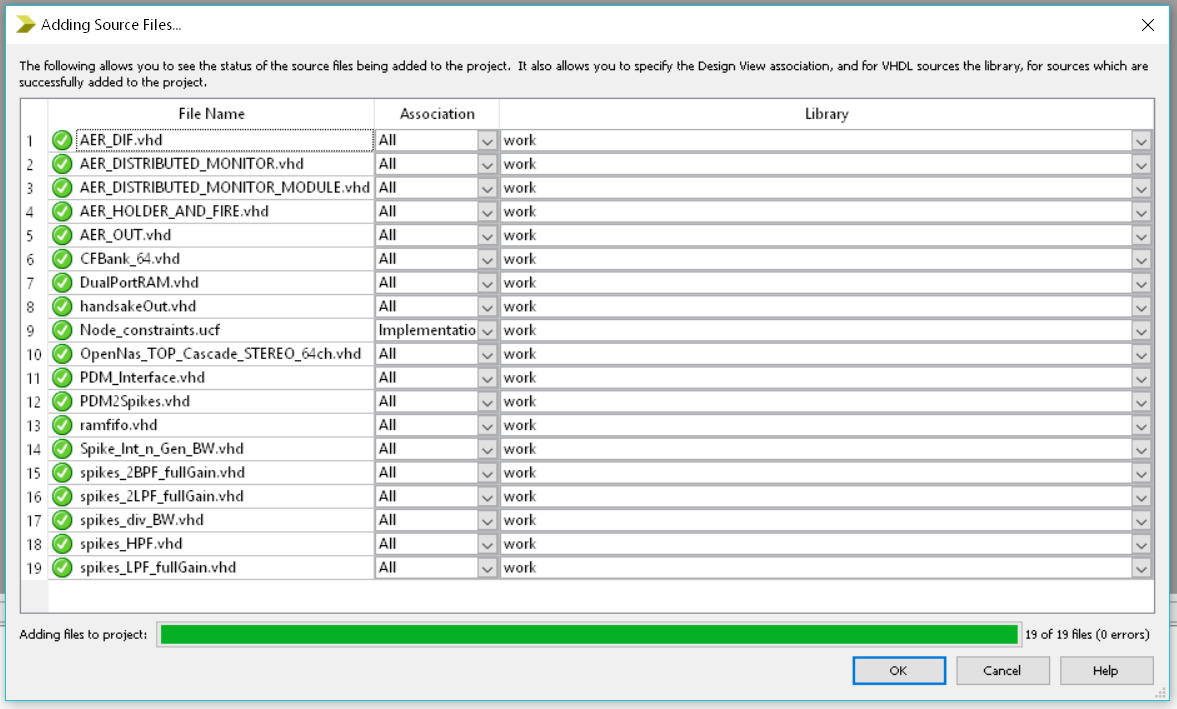
\includegraphics[width=1\textwidth]{images/Img37_AddFilesDone_bis.PNG}
\caption{\label{fig:ISE_accept_add}Selecting the files association.}
\end{figure}

Checking again the project folder in the ISE main window, now we should have a new hierarchy with the included files.

\begin{figure}[H]
\centering
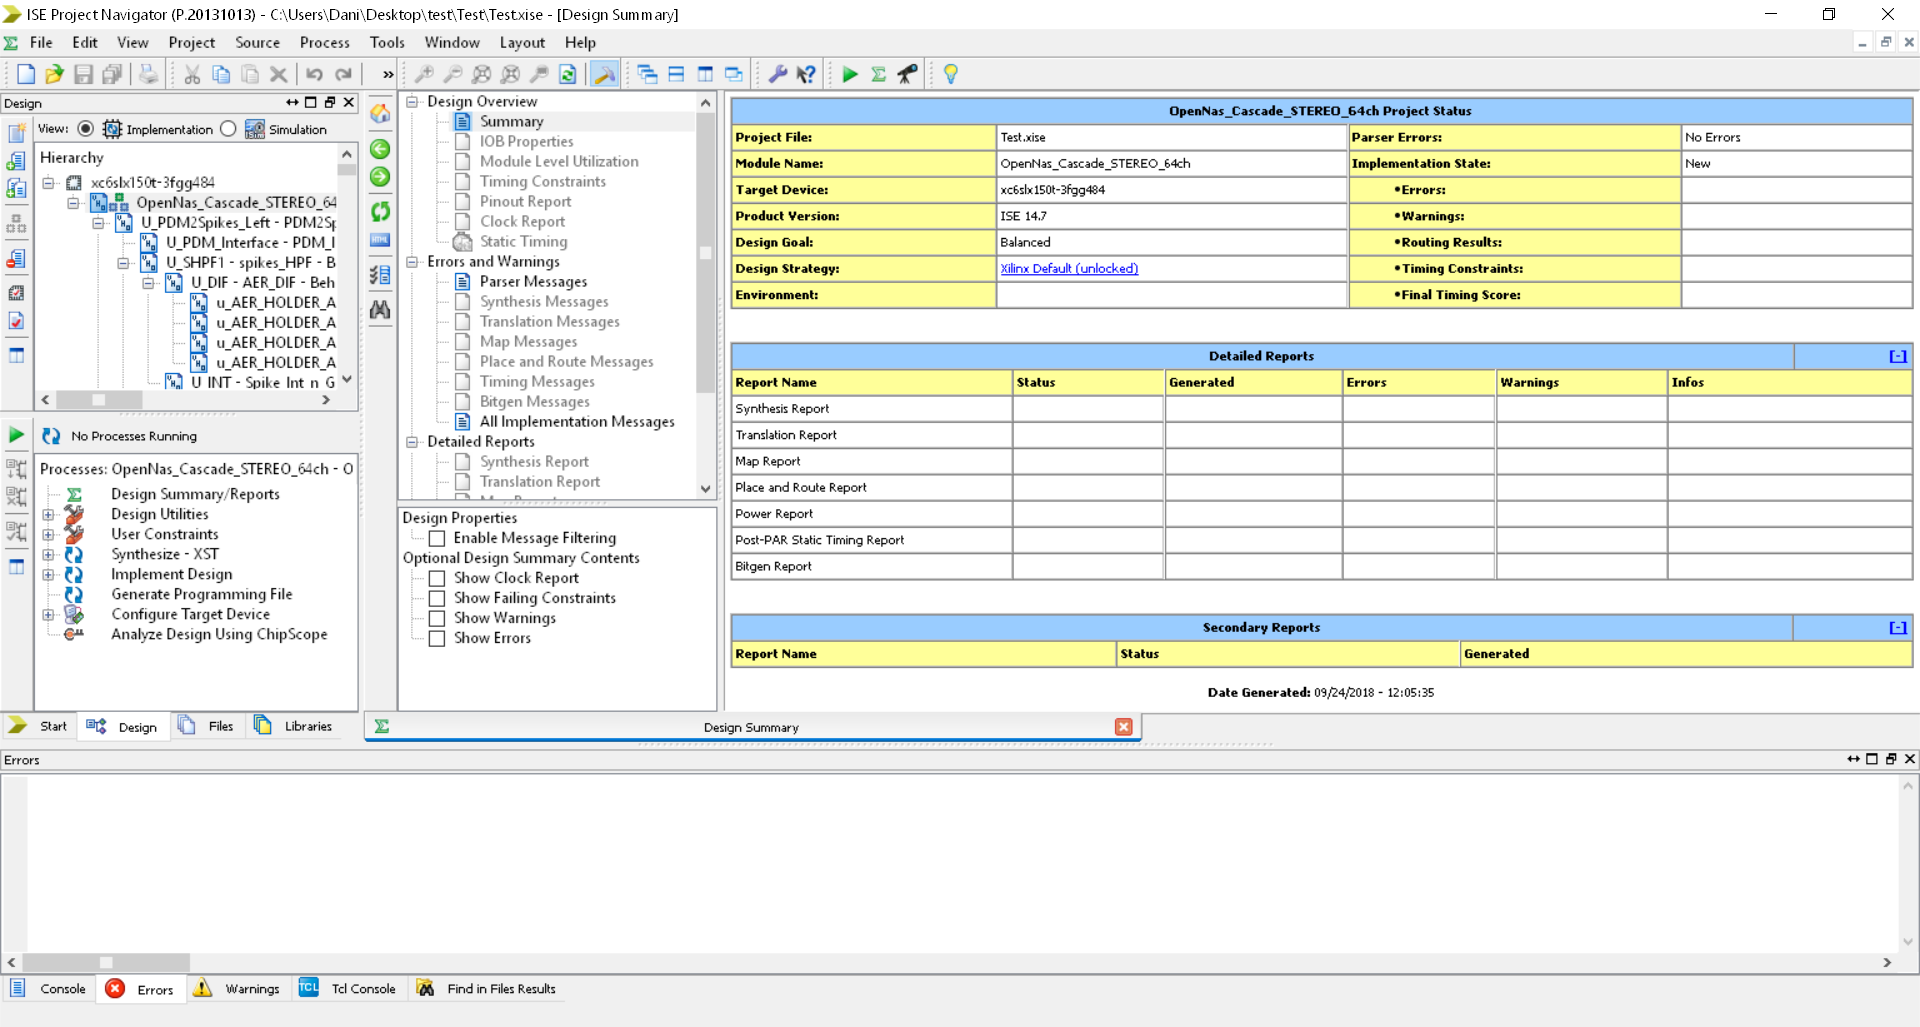
\includegraphics[width=1\textwidth]{images/Img38_ProjectReady.PNG}
\caption{\label{fig:ISE_sources_added}ISE main window after to add the source files.}
\end{figure}

By analyzing that hierarchy, it is easy to identify the three different parts in which we split the NAS architecture: the input (U\_PDM...), the processing block (U\_CFBank\_2or\_64CH), and the output (U\_AER\_Distributed\_Monitor).

\begin{figure}[H]
\centering
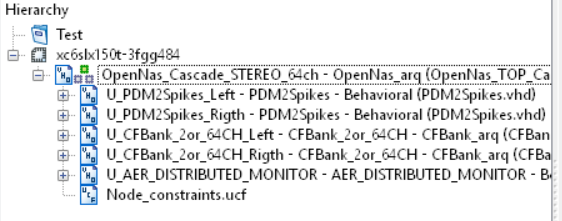
\includegraphics[width=1\textwidth]{images/Img39_Hierarchy.PNG}
\caption{\label{fig:ISE_project_hierarchy}OpenNAS project modules hierarchy.}
\end{figure}

Finally, to start the process of programming file generation, we have to make left click on the top file of the VHDL files hierarchy, and just below some options will appear.

\begin{figure}[H]
\centering
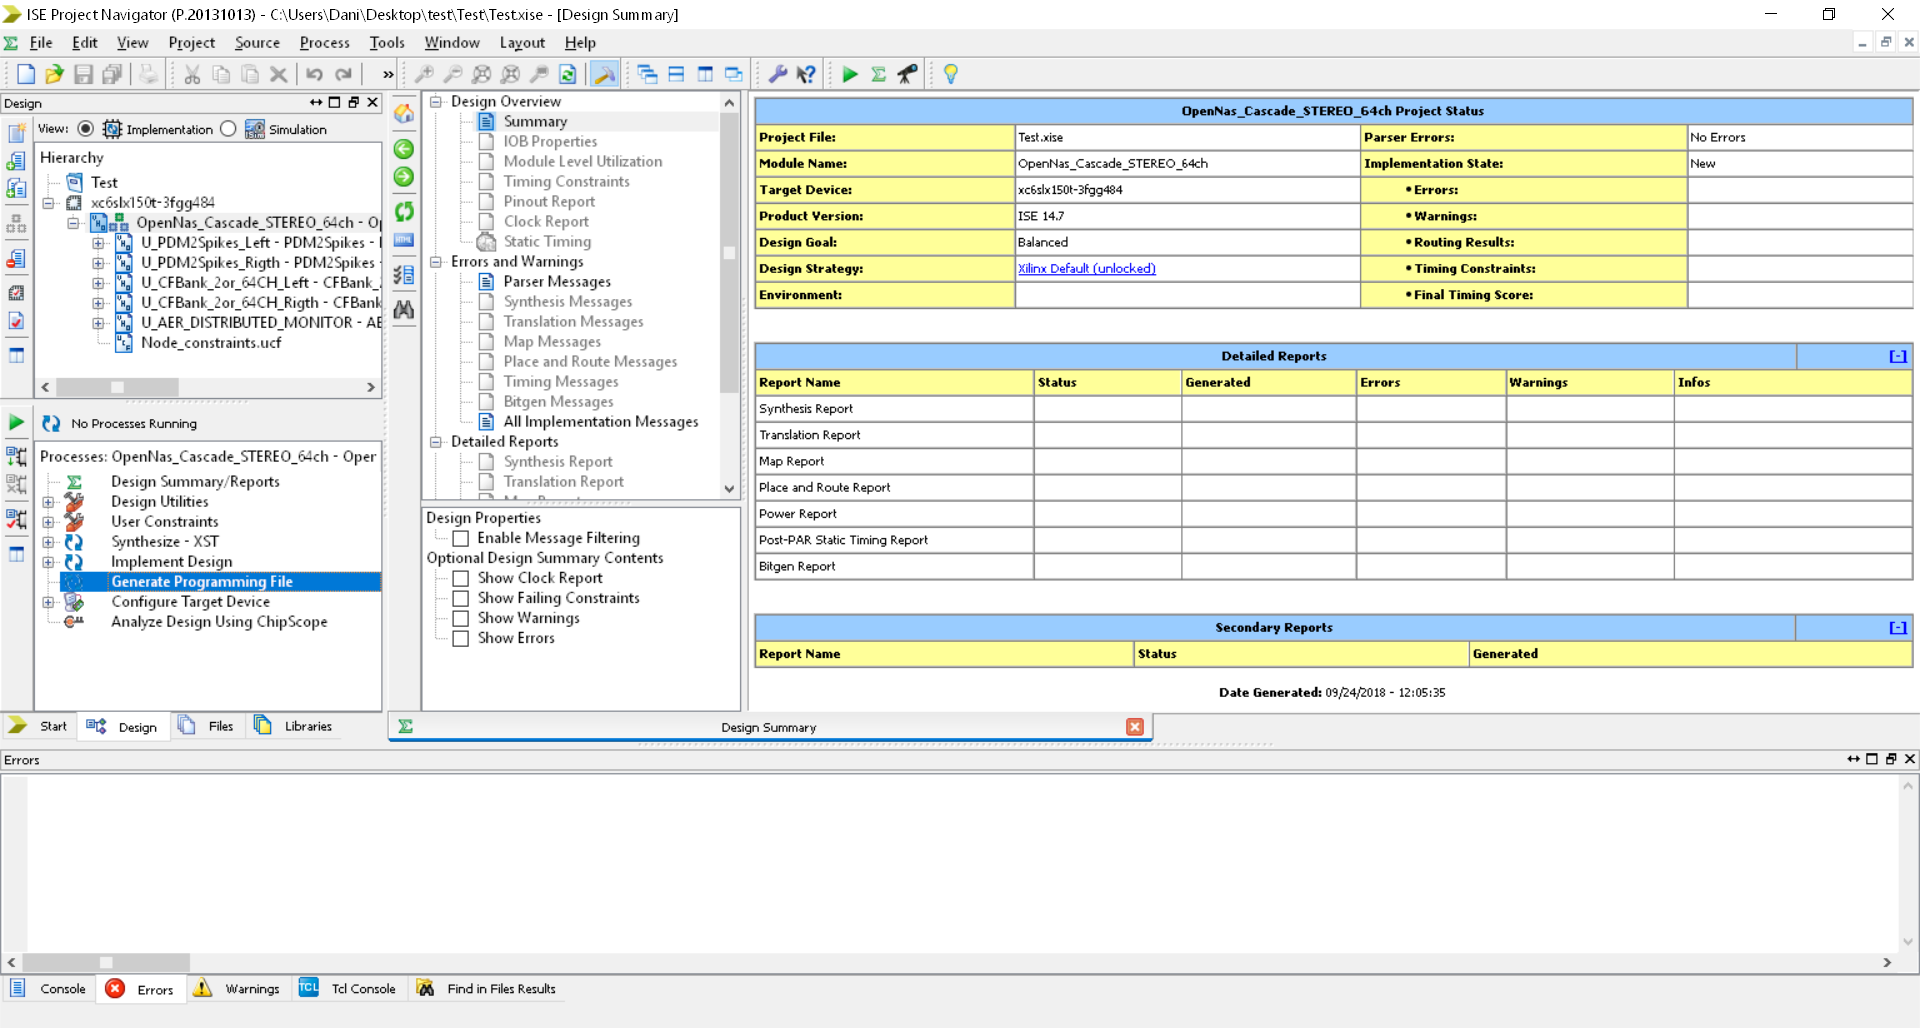
\includegraphics[width=1\textwidth]{images/Img40_GeneratingProgFile.PNG}
\caption{\label{fig:ISE_project_process}Clicking on the top file to show the process menu.}
\end{figure}

Just making double left click on the Generate Programming File option, the entire process will start to running, starting from the synthesis process, implement design process and, at the end, the programming file generation. When the process is finished, you can find the programming file in the project directory, with the extension .bit.

\begin{figure}[H]
\centering
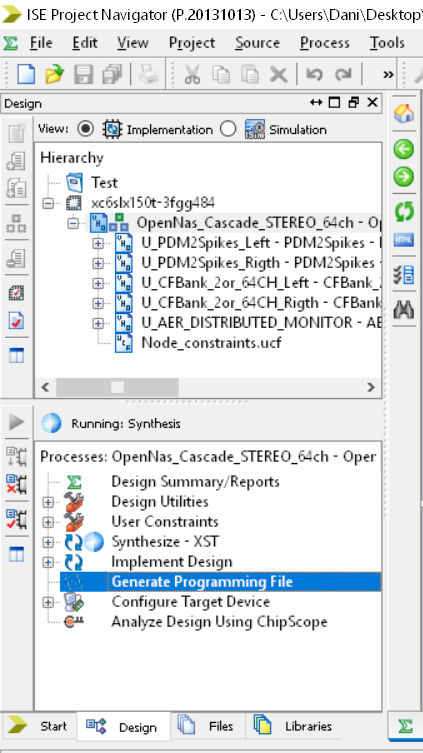
\includegraphics[width=0.5\textwidth]{images/Img41_Running.PNG}
\caption{\label{fig:running_generating_prog_file}Running the Generation Programming File process.}
\end{figure}

Say "need to wait".

%----------------------------------------------------------------------------------------
%	Load bitfile
%----------------------------------------------------------------------------------------

\subsection{Loading bitfile into the AER-Node board}

Once the .bit file has been generated, you need to load it into FPGA. Click on this \textcolor{blue}{ \href{https://github.com/RTC-research-group/AERtools/tree/master/AERNode/NAS/NAS_user_manual}{NAS setup getting started}} link to carry out that process. Moreover, to perform the post-processing step, visit \textcolor{blue}{ \href{https://github.com/jpdominguez/NAVIS-Tool}{NAVIS GitHub website}} \cite{dominguez2017navis}.

\section{Some tricks!}

\begin{itemize}
    \item If you select SpiNNaker v1 as output interface, it would be recommendable to reset both boards in a specific order: push reset button from both boards, then leave the reset button from SpiNNaker, wait until the Ethernet LED's start to blink, and finally leave the reset button from AER-Node board.
\end{itemize}{}

\bibliographystyle{abbrv}
\bibliography{OpenNASTutorial_references.bib} 
% Note the lack of whitespace between the commas and the next bib file.

\end{document}